\documentclass[10pt, aspectratio=169]{beamer}

% Configuration {{{
\usepackage[utf8]{inputenc}
\usepackage[T2A]{fontenc} % T1 for English
\usepackage[english]{babel}

\usepackage{mathtools}
\usepackage{graphicx}
\usepackage{tikz}
\usepackage[multidot]{grffile}
\usepackage[labelsep=period]{caption}
\usepackage{multirow}

\setbeamertemplate{caption}[numbered]
\setbeamertemplate{navigation symbols}{}
\usefonttheme[onlymath]{serif}
\usepackage{DejaVuSansCondensed} % helvet for English
\usetheme{Madrid}

\linespread{1.2}
% }}}

% Definitions {{{
\def\todo#1{\colorbox{orange}{TODO: #1}}

\def\Lb{{\Lambda_b^0}}
\def\Lc{{\Lambda_c^+}}
\def\Lcstar{{\Lambda_c^{*+}}{}}
\def\Lca{{\Lambda_c(2765)^+}}
\def\Lcb{{\Lambda_c(2940)^+}}
\def\LcII{{\Lambda_c(2625)^+}}
\def\LcIII{{\Lambda_c(2880)^+}}
\def\LcIIIother{{\Lambda_c(2765)^+}}
\def\ScI{{\Sigma_c(2455)}}
\def\ScIpp{{\Sigma_c(2455)^{++}}{}}
\def\ScIp{{\Sigma_c(2455)^{+}}{}}
\def\ScIz{{\Sigma_c(2455)^{0}}{}}
\def\ScII{{\Sigma_c(2520)}}
\def\ScIIpp{{\Sigma_c(2520)^{++}}{}}
\def\ScIIp{{\Sigma_c(2520)^{+}}{}}
\def\ScIIz{{\Sigma_c(2520)^{0}}{}}
\def\ScIII{{\Sigma_c(2800)}}
\def\ScIIIpp{{\Sigma_c(2800)^{++}}{}}
\def\ScIIIp{{\Sigma_c(2800)^{+}}{}}
\def\ScIIIz{{\Sigma_c(2800)^{0}}{}}
\def\Sc{{\Sigma_c}}
\def\Scpp{{\Sigma_c^{++}}{}}
\def\Scp{{\Sigma_c^{+}}{}}
\def\Scz{{\Sigma_c^{0}}{}}
\def\Scstar{{\Sigma_c^*}}
\def\Scstarpp{{\Sigma_c^{*++}}{}}
\def\Scstarp{{\Sigma_c^{*+}}{}}
\def\Scstarz{{\Sigma_c^{*0}}{}}
\def\Scoptstar{{\Sigma_c^{(*)}}{}}
\def\Scoptstarpp{{\Sigma_c^{(*)++}}{}}
\def\Scoptstarp{{\Sigma_c^{(*)+}}{}}
\def\Scoptstarz{{\Sigma_c^{(*)0}}{}}
\def\pip{{\pi^+}}
\def\pim{{\pi^-}}
\def\piz{{\pi^0}}
\def\rhop{\rho^+}
\def\rhom{\rho^-}
\def\Kp{{K^+}}
\def\Km{{K^-}}
\def\Kshort{{K_S^0}}
\def\Klong{{K_L^0}}
\def\Kstarz{{K^{*0}}{}}
\def\p{{p}}
\def\Dz{{D^0}}
\def\Dzbar{{\bar{D}^0}}
\def\Dp{{D^+}}
\def\Dsubsm{{\bar{D}_s^0}}
\def\Dsubsp{{D_s^+}}
\def\Dstarp{{D^{*+}}{}}
\def\Dstarz{{D^{*0}}{}}
\def\Dstarzbar{{\bar{D}^{*0}}{}}
\def\Bz{{B^0}}
\def\Bsz{{B_s^0}}
\def\gevcc{{GeV$/c^2$}}
%}}}

% Title and other {{{
\title[Search for CP asymmetry in $b$-hadron decays at LHCb]{
  Search for $b$-hadron decays with CP asymmetry
  \\ and its measurement at the LHCb detector
}
\author[Kerim Guseynov]{
  Kerim Guseynov
  \vskip 1ex
  \scriptsize
  Based on analyses by the LHCb Collaboration: \\
  Observation of the suppressed $\Lambda_{b}^{0}\ensuremath{\rightarrow}Dp{K}^{\ensuremath{-}}$ decay with $D\ensuremath{\rightarrow}{K}^{+}{\ensuremath{\pi}}^{\ensuremath{-}}$ and measurement of its $CP$ asymmetry,
  \\ Phys.Rev. D104 (2021) 112008 \\
  Model-independent measurement of the CKM angle $\gamma$ using $\Bz\to D\Kstarz$ decays with $D\to\Kshort\pip\pim$ and $\Kshort\Kp\Km$,
  \\ JHEP 06 (2016) 131 \\
  Updated search for $B_c$ decays to two charm mesons,
  JHEP 12 (2021) 117 \\
}
\institute[MSU]{
  Faculty of Physics \\ Moscow State University
}
\date{April 19, 2023}
%}}}

\begin{document}

\frame[plain]{\titlepage}

\begin{frame}[label=introduction]%{{{
  \frametitle{Introduction}

  \begin{itemize}
    \item The CP asymmetry is responsible for the matter/antimatter 
      imbalance in the Universe.
    \item While the Standard Model has sources of CP violation, they are 
      not large enough to account for the observed matter dominance.
      \\ Nonetheless, their measurement is still important.
    \item The main source is the CKM quark mixing matrix.
      \\ Its least precise measurement is the $\gamma$ angle.
    \item $B^-\to DK^-$ and some others are thoroughly investigated, but 
      there are decays with better interfering amplitudes.
    \item Measurements of CP violation in specific decays also test 
      theoretical calculation.
    \item Search for new complex decays with interference may reveal new 
      physics.
  \end{itemize}
\end{frame}%}}}

\begin{frame}[label=mixing]%{{{
  \frametitle{Cabibbo Kobayashi Maskawa matrix. Quark mixing. Meson mixing}
  \centering
  \parbox{.45\linewidth}{
    \large
    \[
      \begin{bmatrix}d'\\s'\\b'\end{bmatrix} =
      \begin{bmatrix}
        V_{\mathrm {ud} } & V_{\mathrm {us} } & V_{\mathrm {ub} } \\
        V_{\mathrm {cd} } & V_{\mathrm {cs} } & V_{\mathrm {cb} } \\
        V_{\mathrm {td} } & V_{\mathrm {ts} } & V_{\mathrm {tb} } \\
      \end{bmatrix}
      \begin{bmatrix}d\\s\\b\end{bmatrix}
    \]

    \normalsize \vskip 3ex
    Quarks are not the same for the strong and weak interactions
    \vskip 1ex
    Unnoticed in normal decays like $n\to p e^-\bar{\nu}_e$
    \vskip 1ex
    Kaon mixing: $K^0$, $\bar{K}^0$, $\to$ $\Kshort$, $\Klong$
    \vskip 1ex
    Same for other neutral mesons: $D^0$, $B^0$, $B_s^0$
  } \parbox{.5\linewidth}{
    \centering
    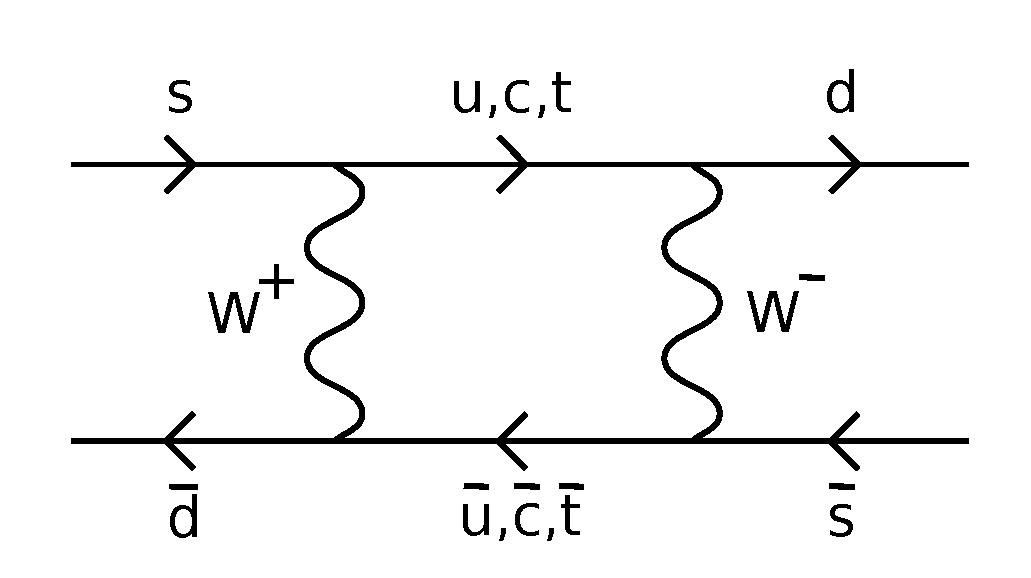
\includegraphics[width=.75\linewidth]{figures/lect/Kaon-mixing-1}
    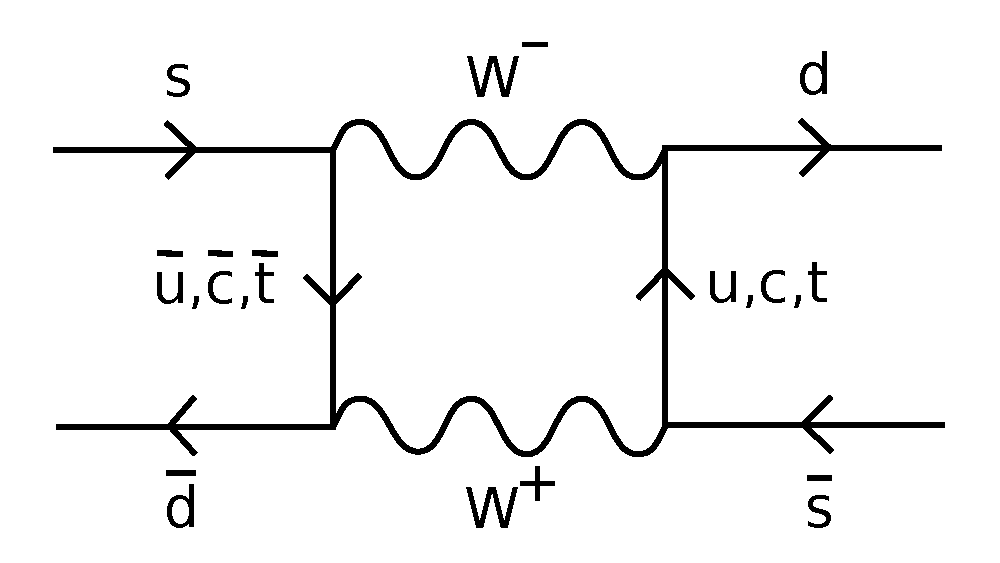
\includegraphics[width=.75\linewidth]{figures/lect/Kaon-mixing-2}
    \vfill
    Neutral kaon mixing
  }
\end{frame}%}}}

\begin{frame}[label=diagrams]%{{{
  \frametitle{Decays with possible CP asymmetry. Interference}
  \vfill
  \centering
  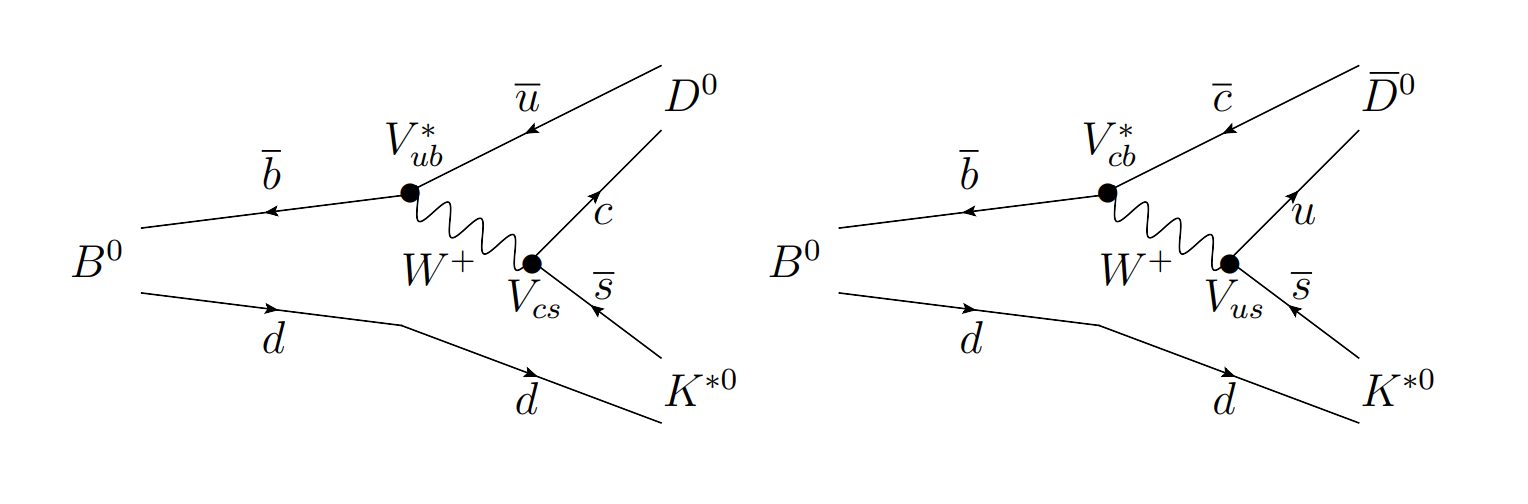
\includegraphics[width=.7\linewidth]{figures/lect/B2DKstar-diagram}
  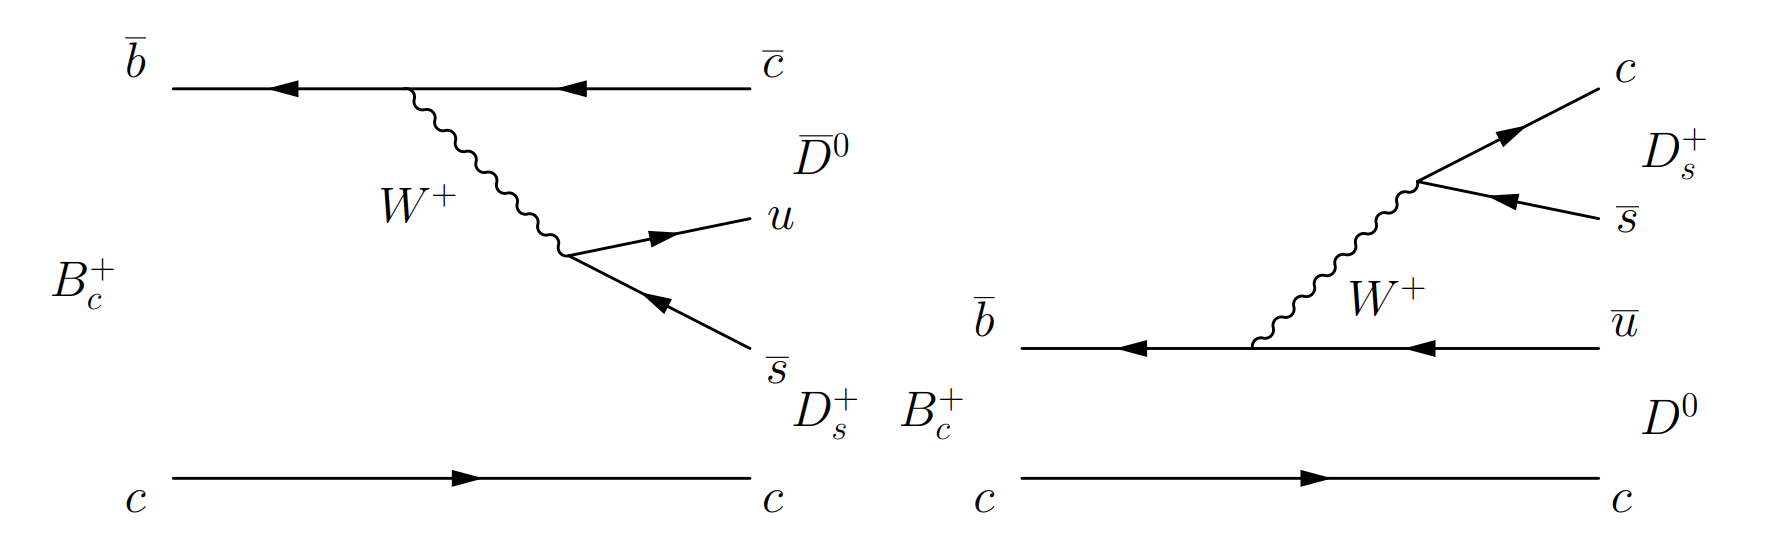
\includegraphics[width=.7\linewidth]{figures/lect/Bc2DD-diagram}
\end{frame}%}}}

\begin{frame}[label=lhcb]%{{{
  \frametitle{The LHCb detector at the LHC}
  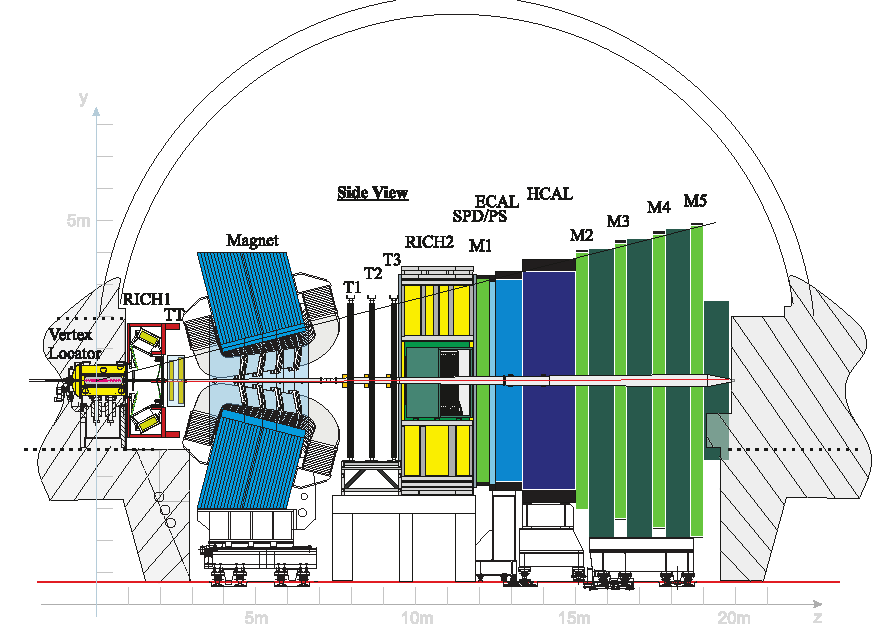
\includegraphics[width=.59\linewidth]{figures/conf/lhcb-detector}
  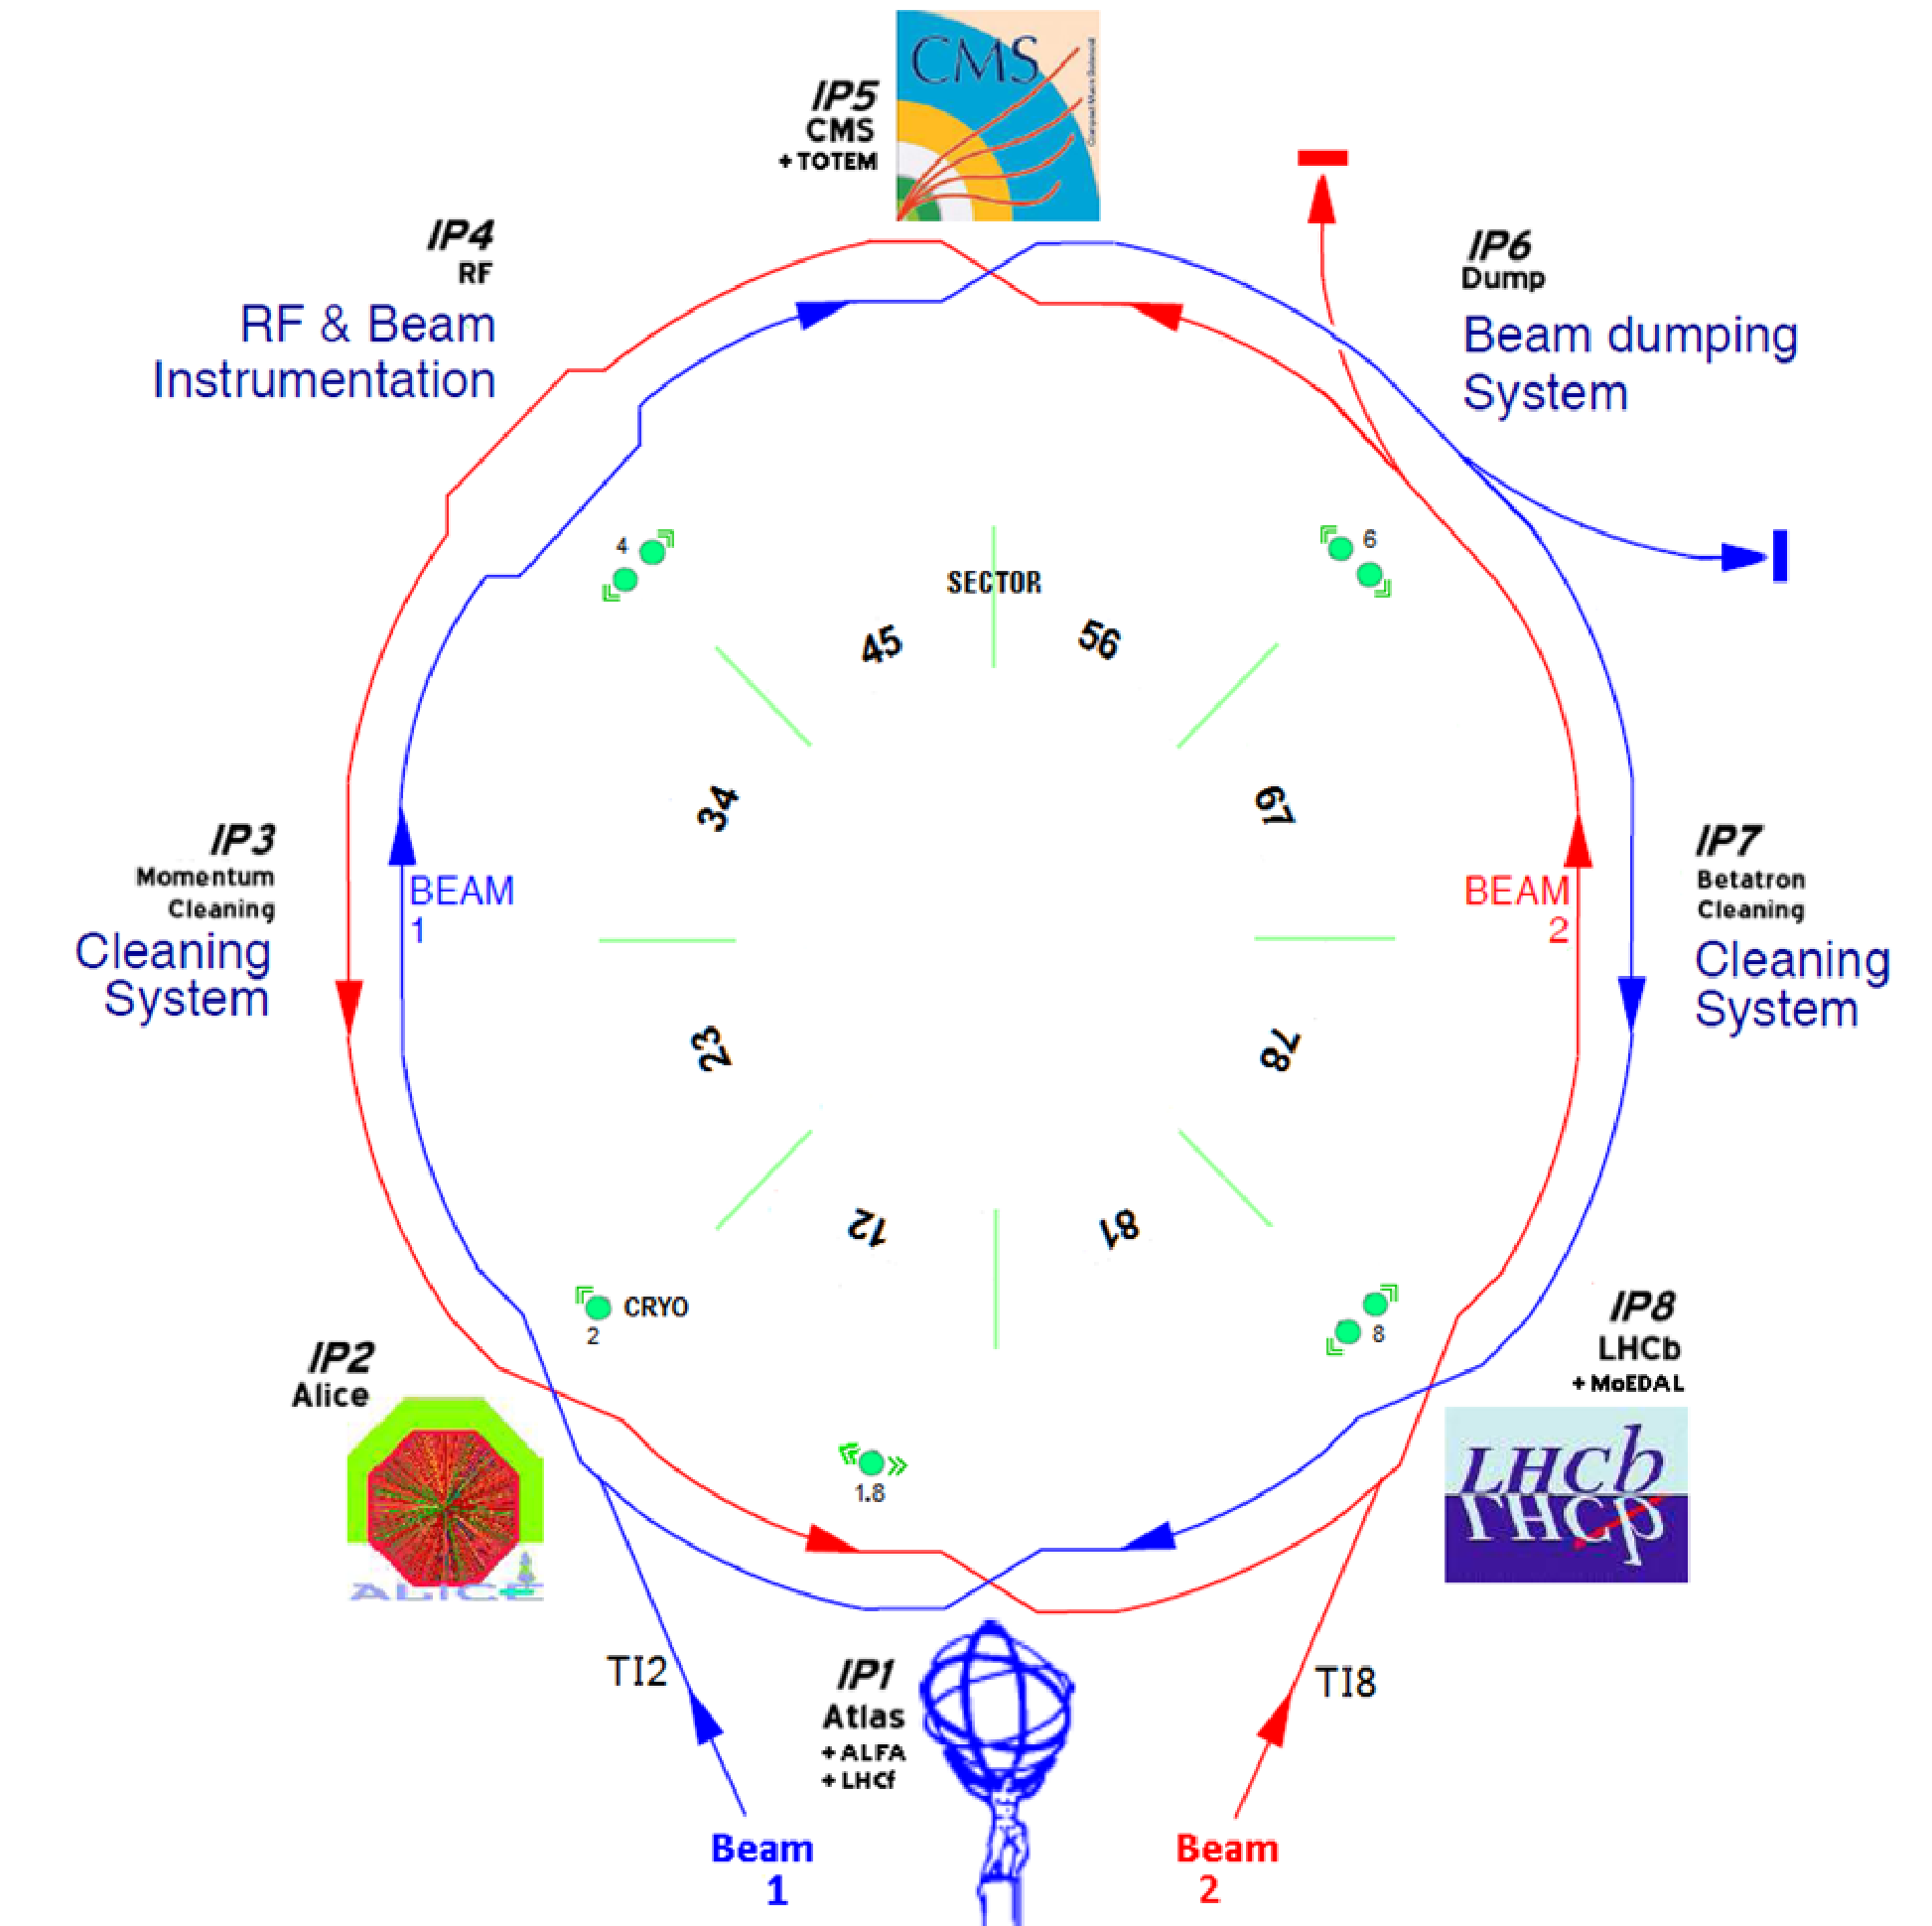
\includegraphics[width=.39\linewidth]{figures/conf/lhc-ring}
\end{frame}%}}}

\begin{frame}[label=analyses]%{{{
  \frametitle{Measurements}
  \centering
  \begin{itemize}
    \item Ratio of decays and the asym. of the less probable one:
      $\Lb\to D(\to K^\mp\pi^\pm)\p\Km$
      \parbox{1\linewidth}{
        \centering
        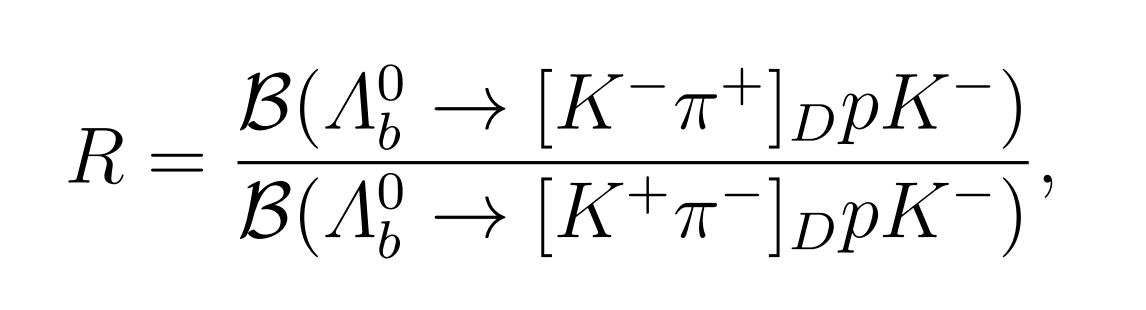
\includegraphics[width=.3\linewidth]{figures/lect/Lb2DpK-ratio} \\
        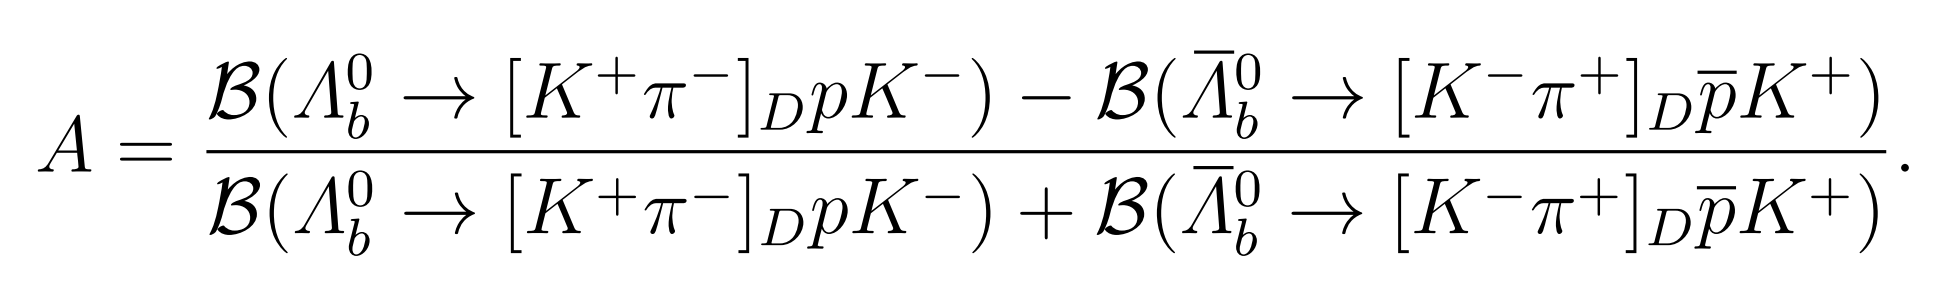
\includegraphics[width=.6\linewidth]{figures/lect/Lb2DpK-asym}
      }

    \item Event distribution by momenta and measurements of interference 
      parameters: \large
      \[ B^0 \to D \Kstarz, \qquad
      D \to \Kshort\pip\pim \text{ or } \Kshort\Kp\Km\]
      \normalsize

    \item Search for decays of $B_c^+$ into
      $D_s^{+}\bar{D}^{0}$,
      $D_s^{+}{D}^{0}$,
      $D^{+}\bar{D}^{0}$,
      $D^{+}{D}^{0}$,
      $D_s^{*+}{D}^{0}$,
      $D_s^{+}{D}^{*0}$, etc.
  \end{itemize}
\end{frame}%}}}

\begin{frame}[label=selection]%{{{
  \frametitle{Event selection}

  \begin{itemize}
    \item Cuts on kinematic variables:
      $p_T$, $\eta$, distance from the $pp$ interaction, \ldots,
    \item Cuts on particle identification parameters and event 
      reconstruction variables,
    \item Exclusion of specific troublesome cases by cutting out 
      kinematic regions,
    \item Usage of neural networks for further improvement of signal 
      purity and quality.
  \end{itemize}

  \centering \vfill
  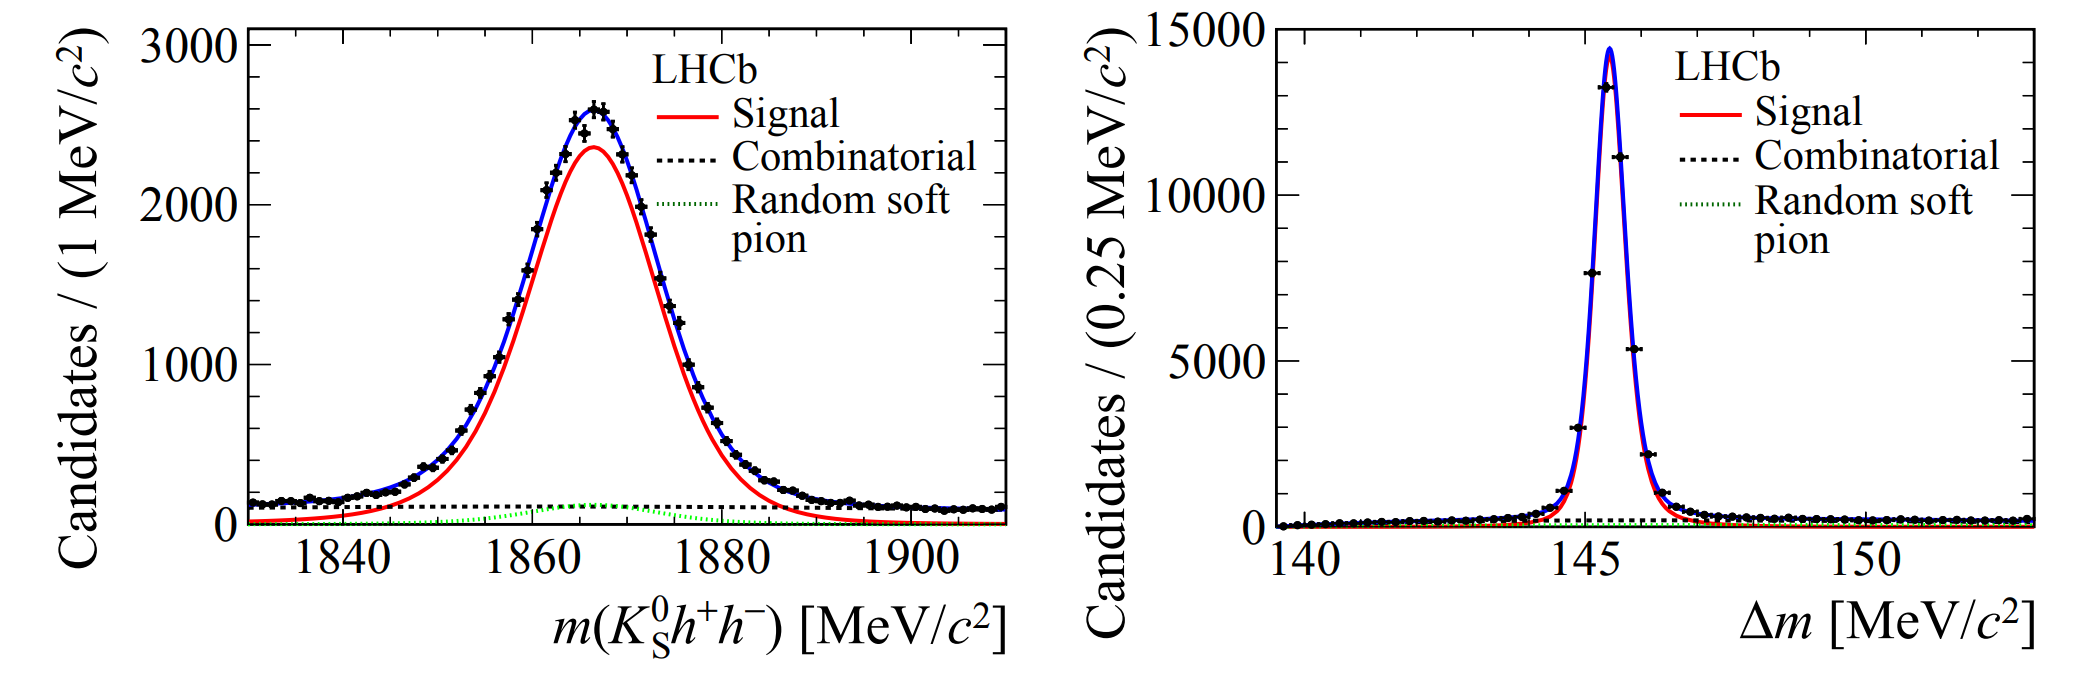
\includegraphics[width=.8\linewidth]{figures/lect/B2DKstar-pointless}
\end{frame}%}}}

\begin{frame}[label=Lb2DpK-fit]%{{{
  \frametitle{Invariant mass spectrum model and fit: $\Lb\to Dp\Km$}
  \centering
  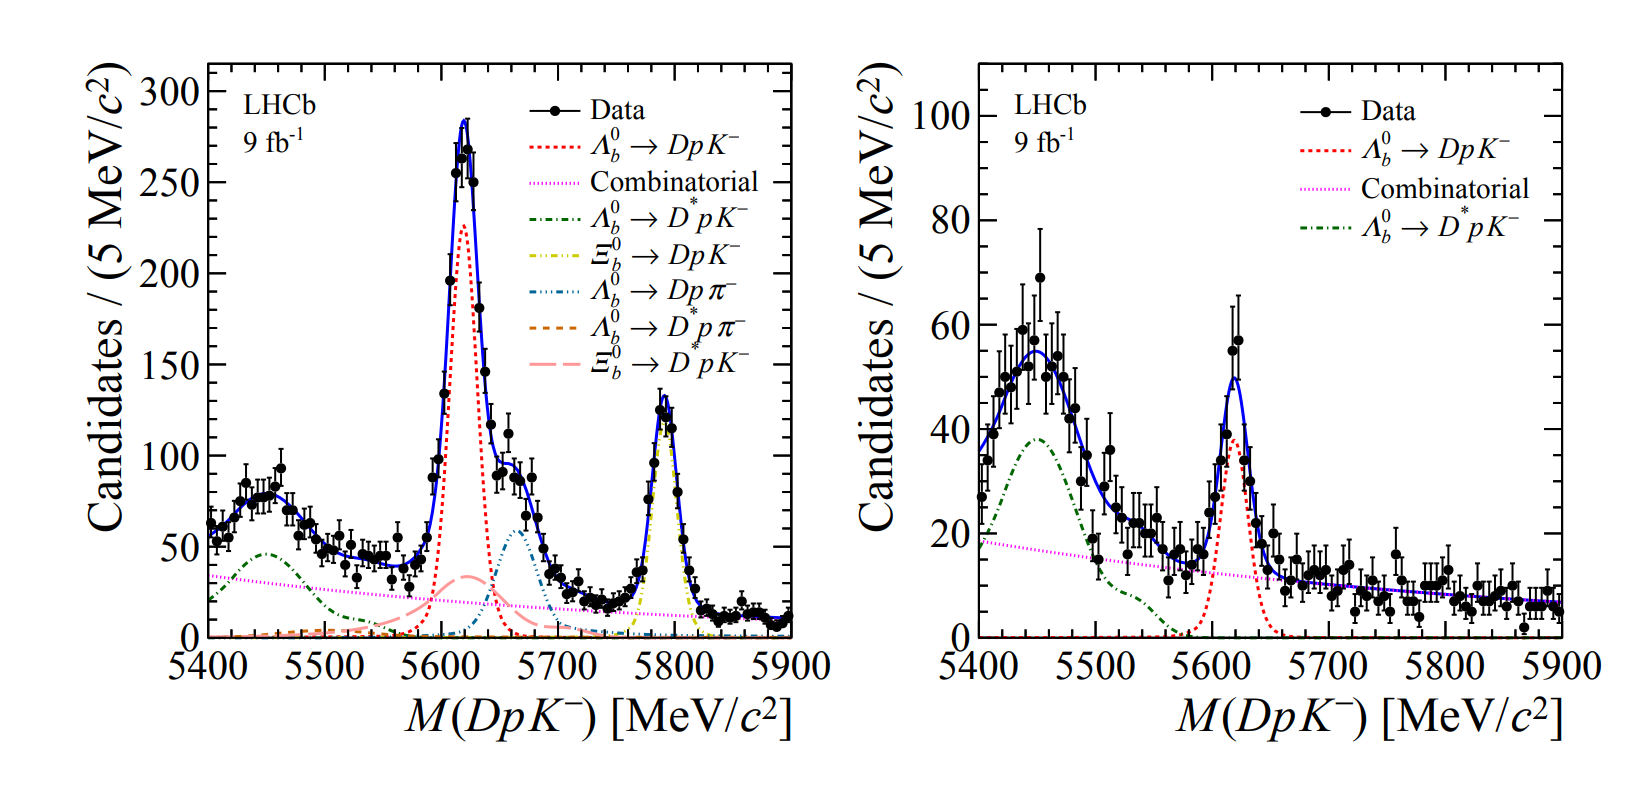
\includegraphics[width=.45\linewidth]{figures/lect/Lb2DpK-full}
  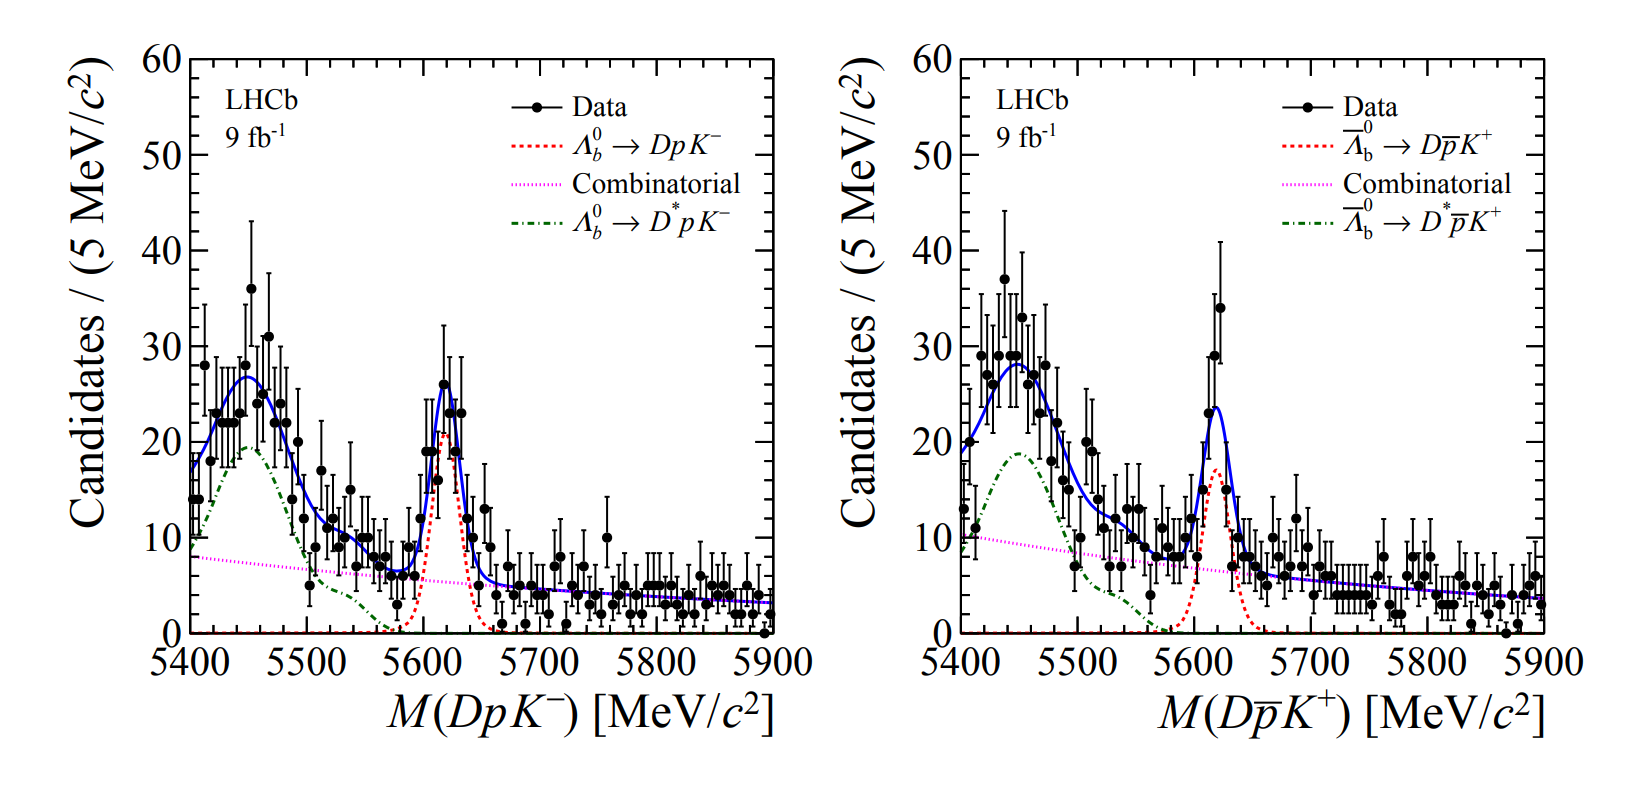
\includegraphics[width=.45\linewidth]{figures/lect/Lb2DpK-asym-full}
  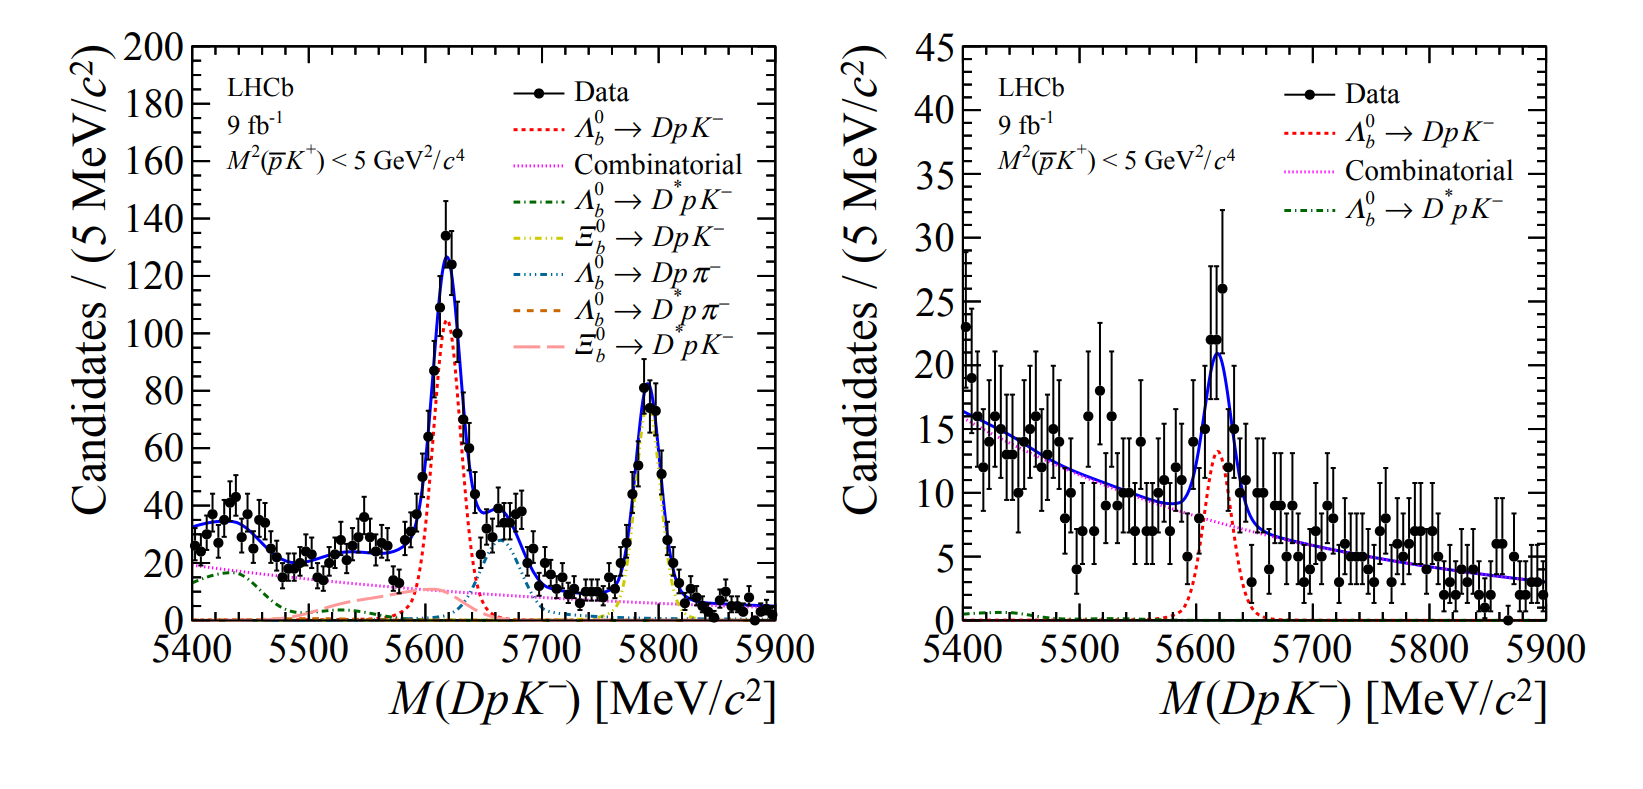
\includegraphics[width=.45\linewidth]{figures/lect/Lb2DpK-restricted}
  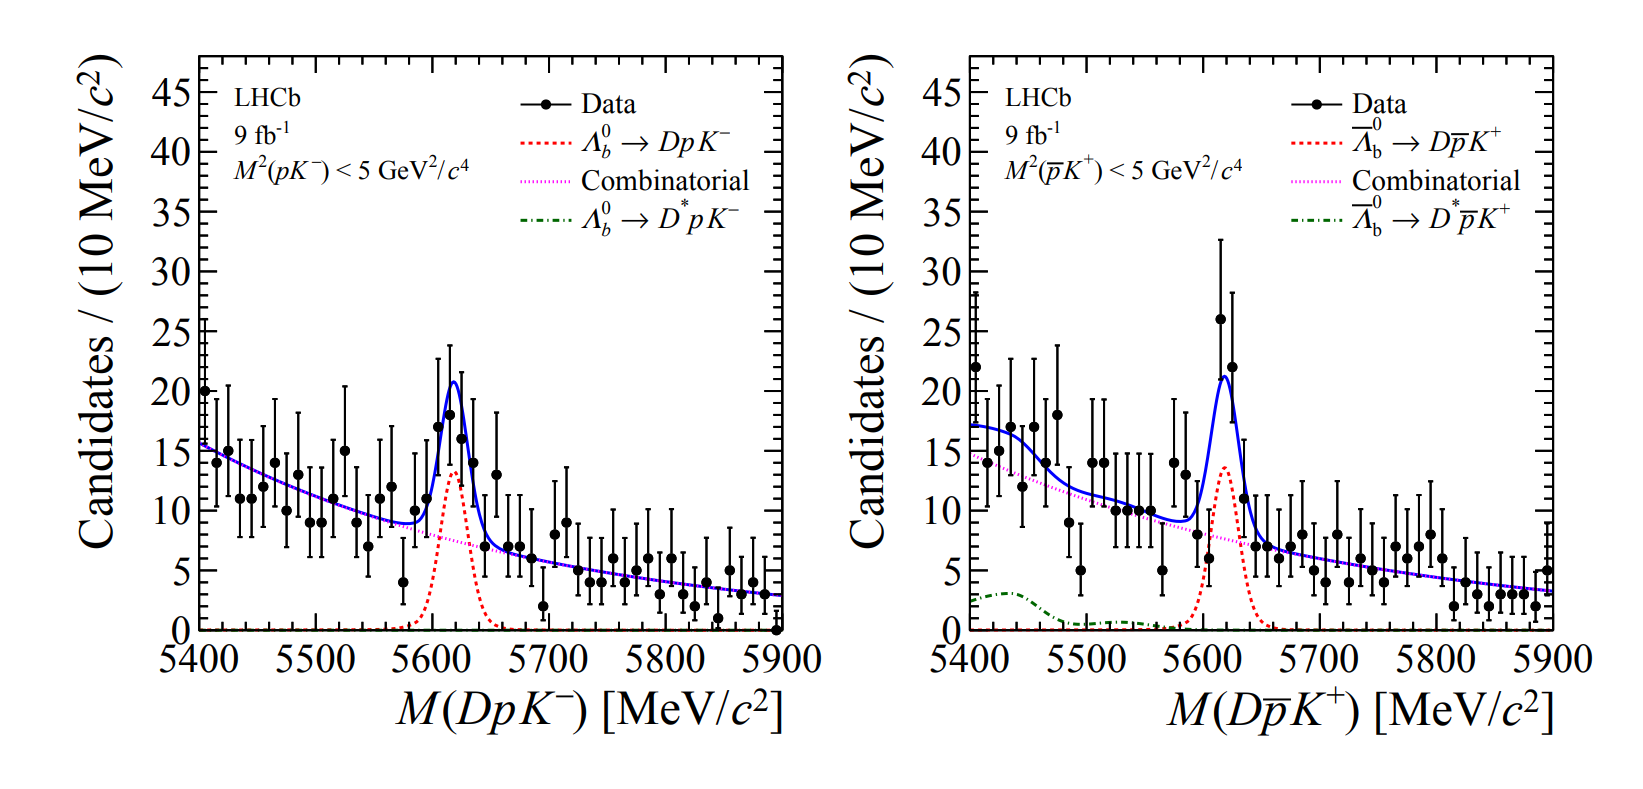
\includegraphics[width=.45\linewidth]{figures/lect/Lb2DpK-asym-restricted}
  \vskip -1ex
  \parbox{.22\linewidth}{\centering $D\to\Km\pip$}
  \parbox{.22\linewidth}{\centering $D\to\Kp\pim$}
  \parbox{.22\linewidth}{\centering $\Lb$}
  \parbox{.22\linewidth}{\centering $\bar{\Lambda}_b^0$}
\end{frame}%}}}

\begin{frame}[label=B2DKstar-fit]%{{{
  \frametitle{Invariant mass spectrum model and fit: $B^0\to D\Kstarz$}
  \centering
  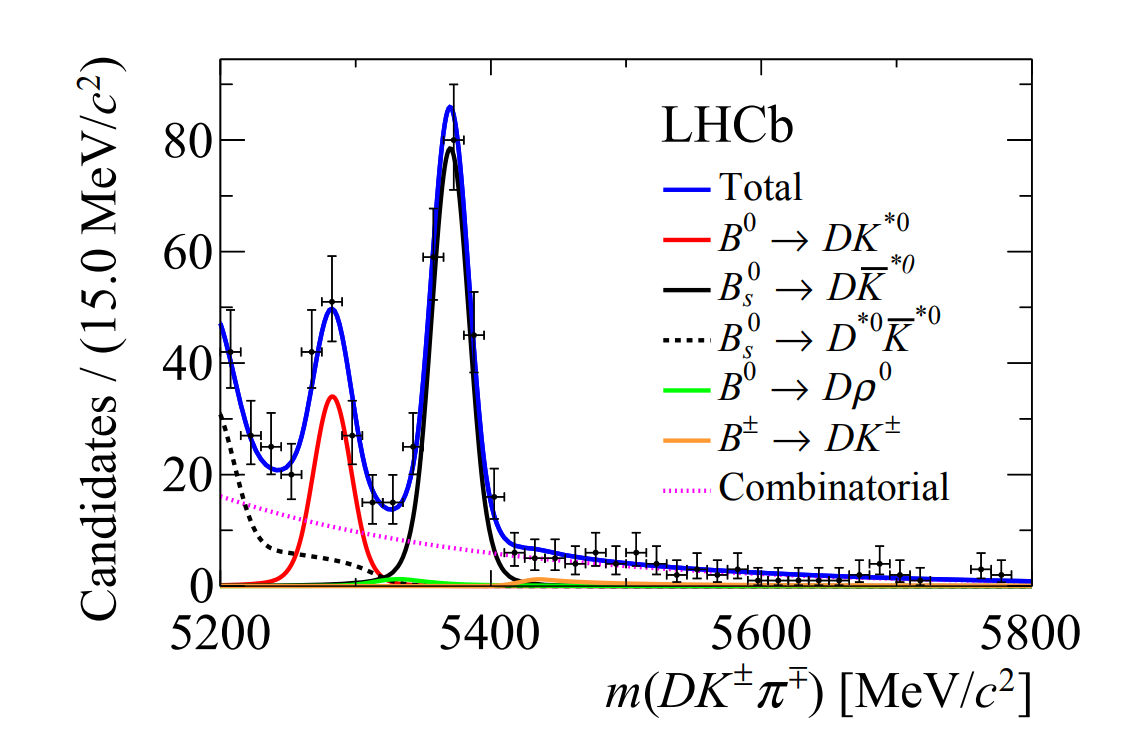
\includegraphics[width=.45\linewidth]{figures/lect/B2DKstar-fit-Kspipi}
  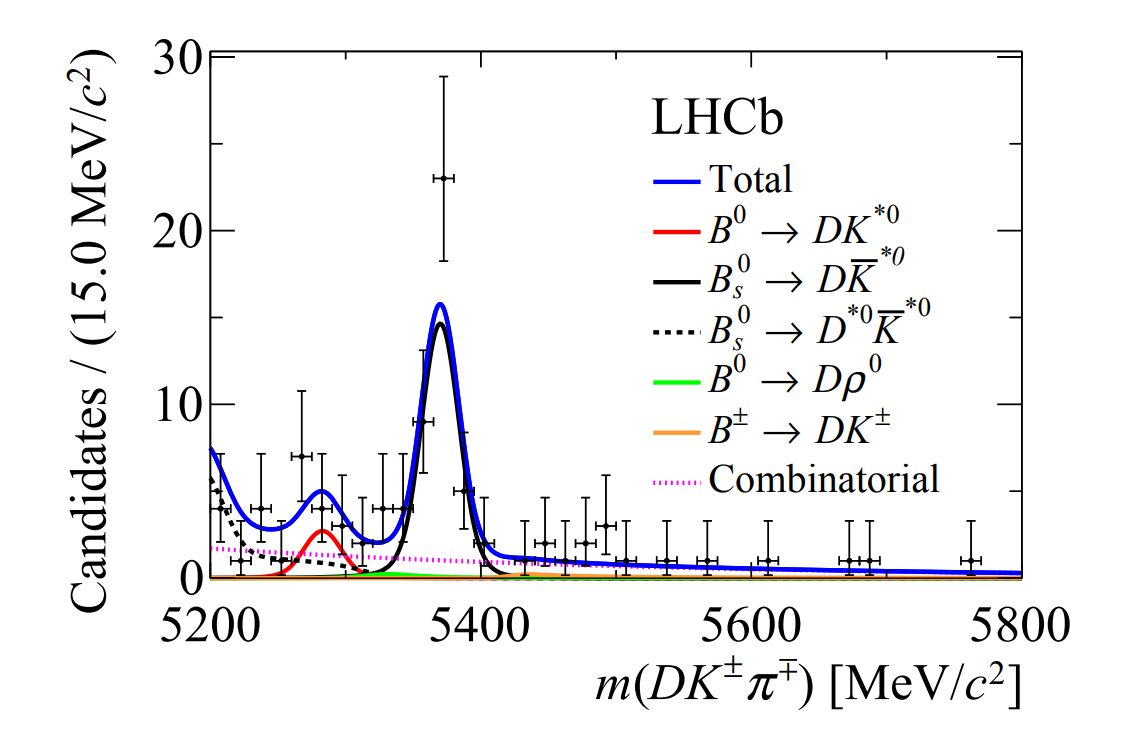
\includegraphics[width=.45\linewidth]{figures/lect/B2DKstar-fit-KsKK}
  \vskip -1ex
  \parbox{.45\linewidth}{\centering $D\to\Kshort\pip\pim$}
  \parbox{.45\linewidth}{\centering $D\to\Kshort\Kp\Km$}
\end{frame}%}}}

\begin{frame}[label=Bc2DD-fit]%{{{
  \frametitle{Invariant mass spectrum model and fit: $B_c^+\to DD$}
  \centering
  \parbox{.54\linewidth}{
    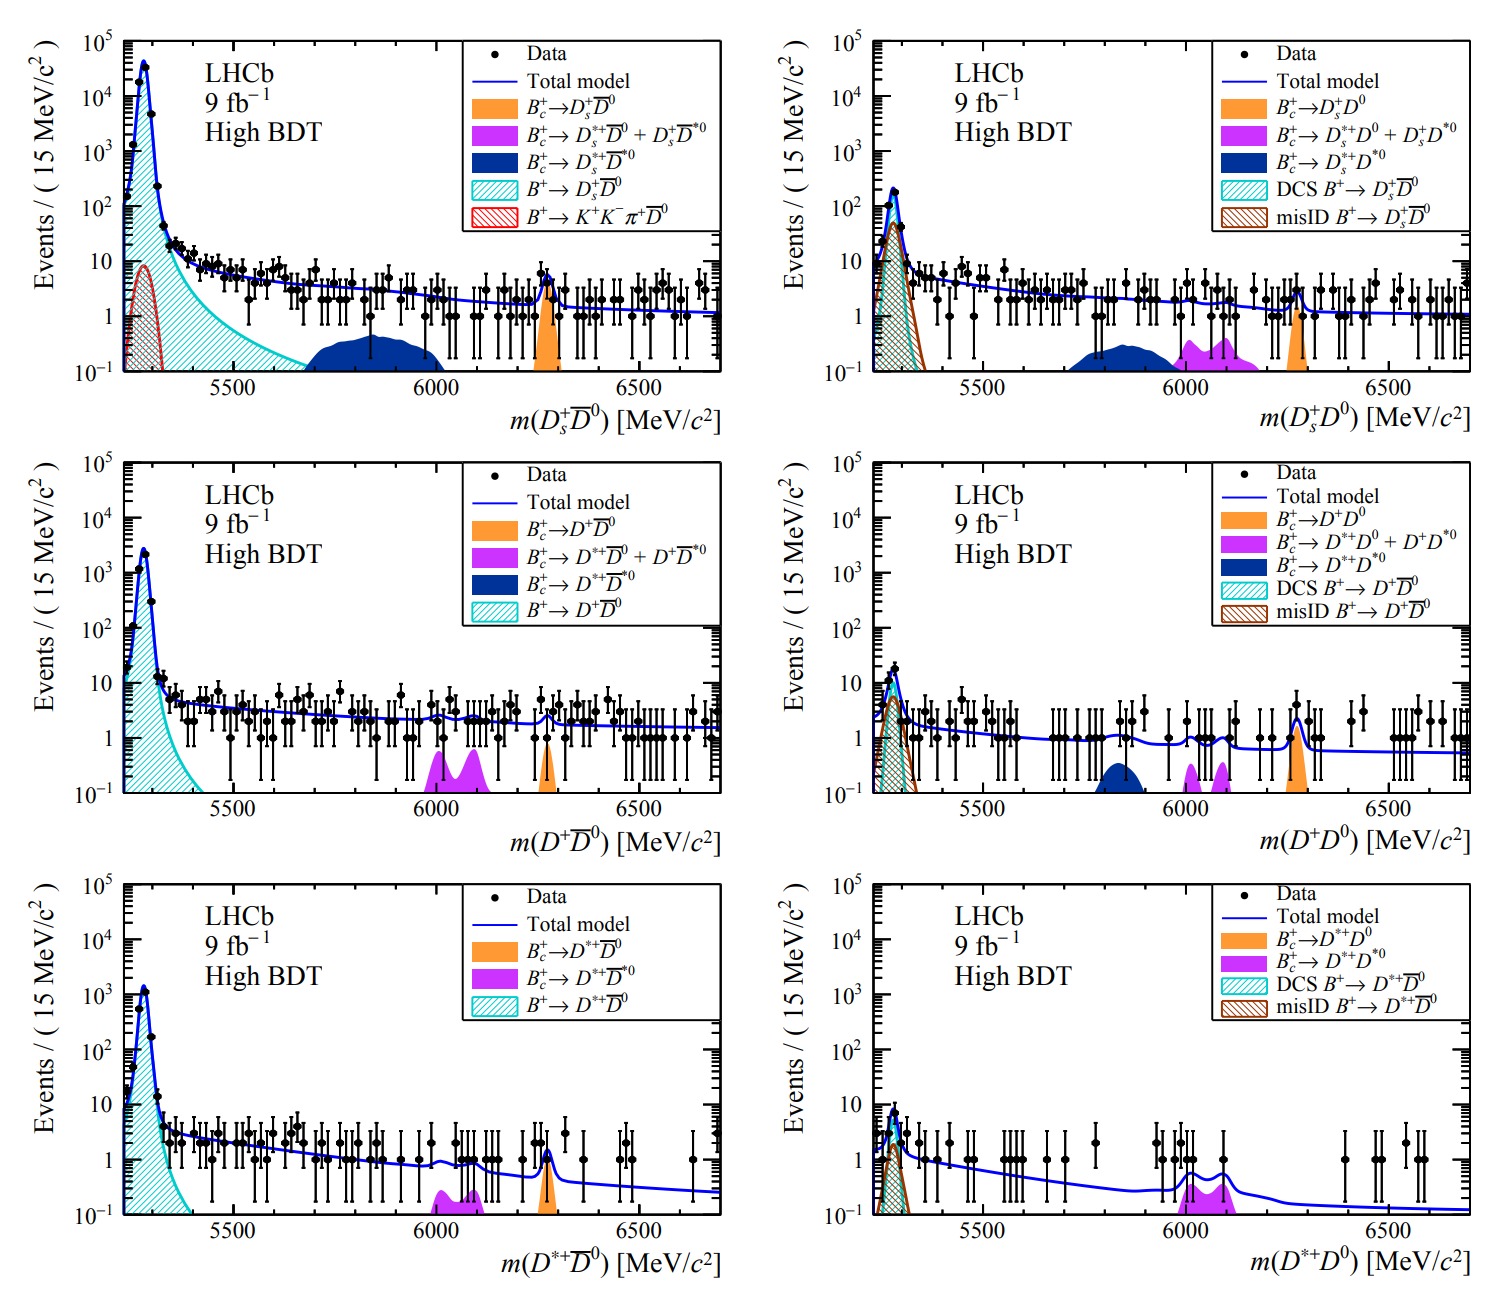
\includegraphics[width=\linewidth]{figures/lect/Bc2DD-fit-all}
  }
  \parbox{.45\linewidth}{
    \centering
    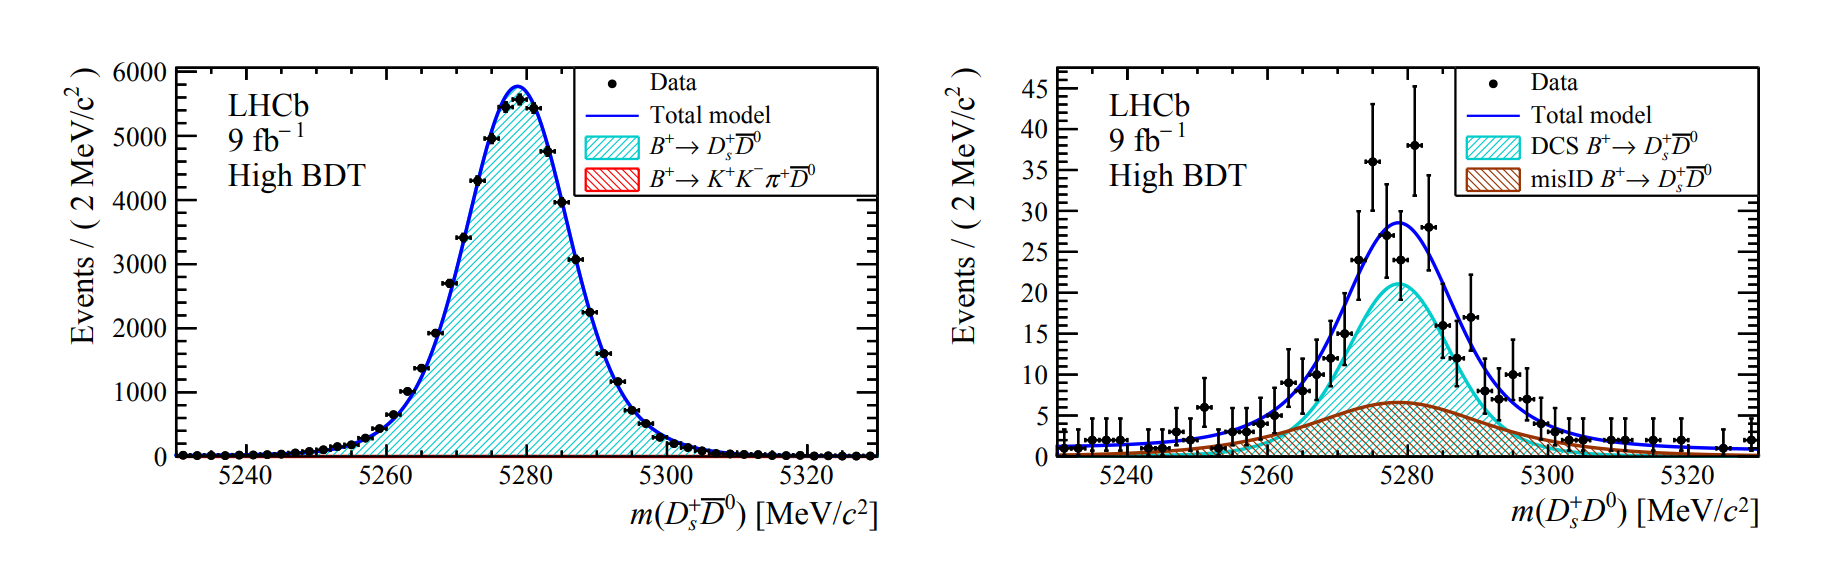
\includegraphics[width=\linewidth]{figures/lect/Bc2DD-fit-lower}
    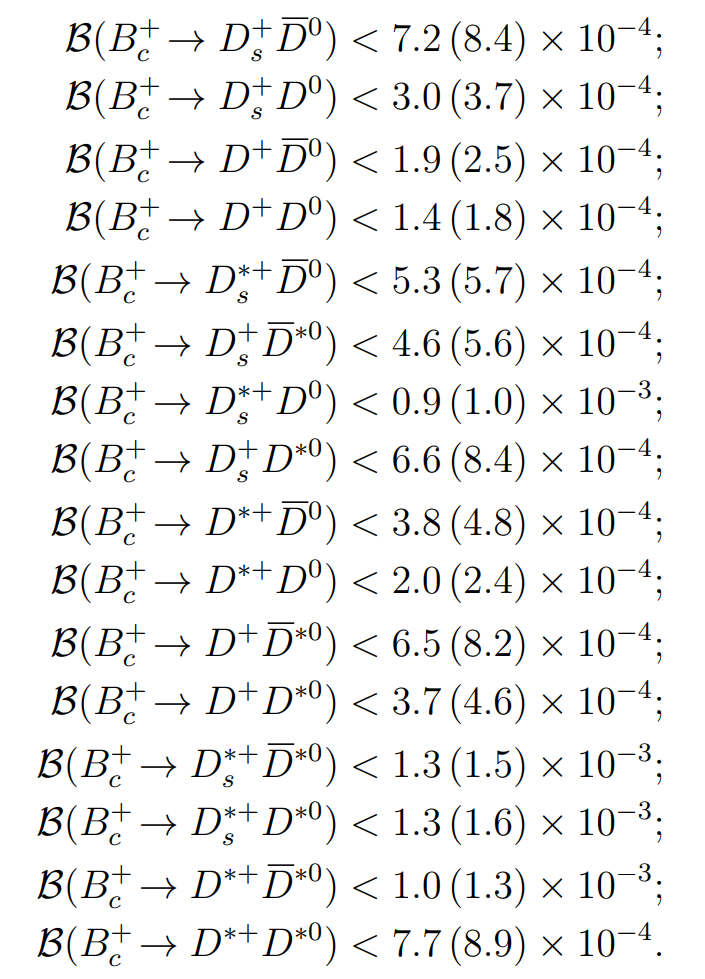
\includegraphics[width=.5\linewidth]{figures/lect/Bc2DD-results}
  }
\end{frame}%}}}

\begin{frame}[label=Lb2DpK-Dalitz-eff]%{{{
  \frametitle{Dalitz plot for $\Lb\to Dp\Km$: resonances, efficiency, 
  measurements}
  \centering
  \parbox{.75\linewidth}{
    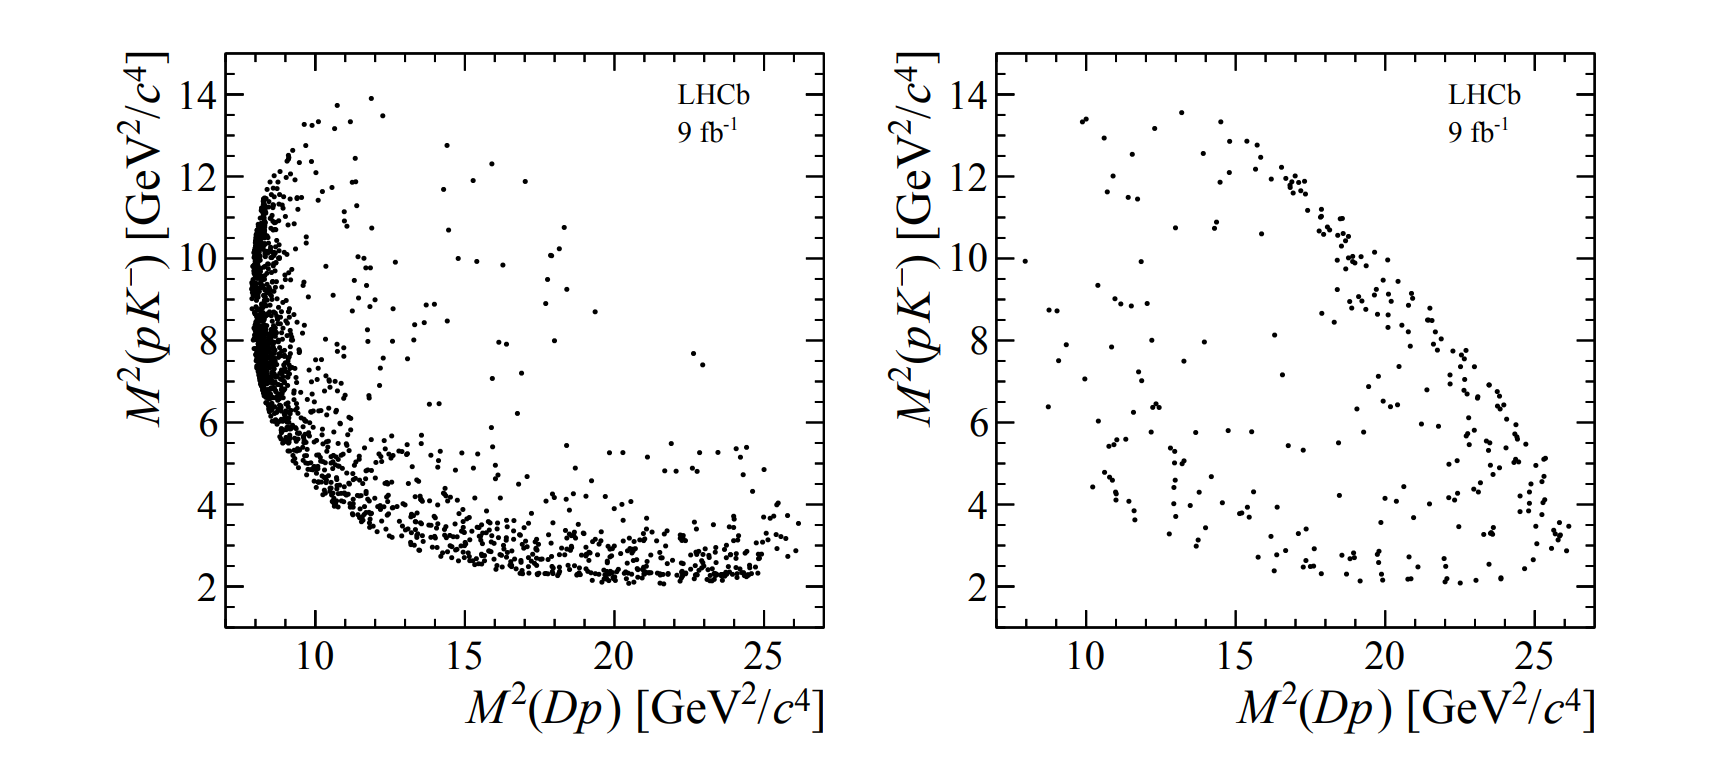
\includegraphics[width=\linewidth]{figures/lect/Lb2DpK-Dalitz}
    \vskip -2ex
    \parbox{.5\linewidth}{\centering $D\to\Km\pip$}
    \parbox{.5\linewidth}{\centering $D\to\Kp\pim$}
  } \parbox{.24\linewidth}{
    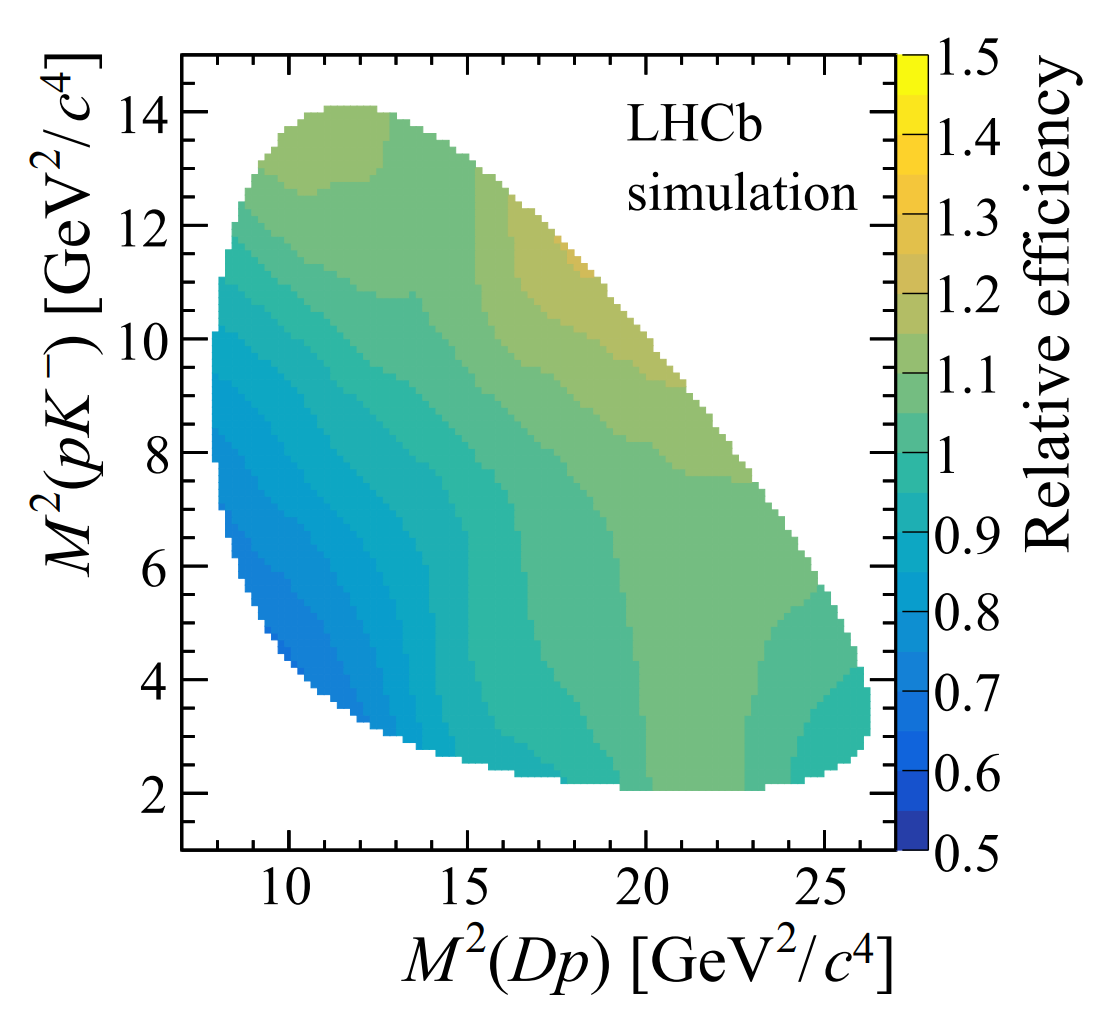
\includegraphics[width=\linewidth]{figures/lect/Lb2DpK-eff}
  }
  \vfill
  \parbox{.45\linewidth}{
    \centering Full:
    \parbox{.65\linewidth}{
      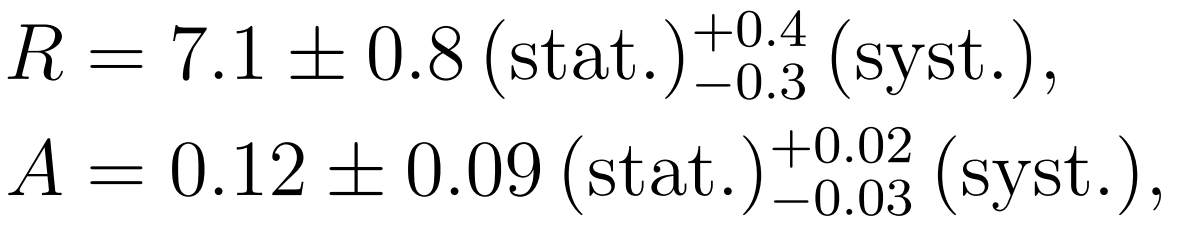
\includegraphics[width=\linewidth]{figures/lect/Lb2DpK-results-full}
    }
  } \parbox{.45\linewidth}{
    \centering Restricted:
    \parbox{.65\linewidth}{
      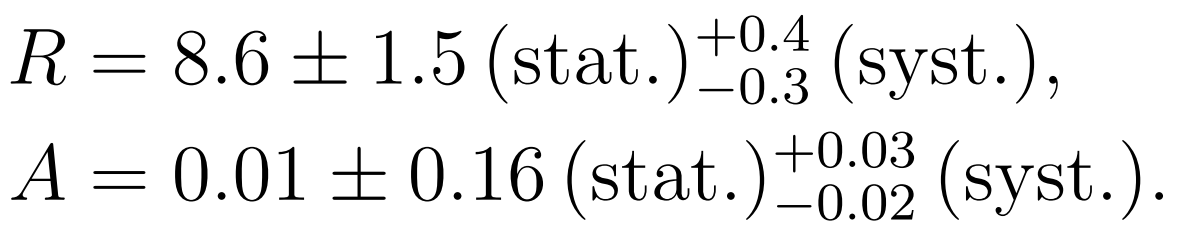
\includegraphics[width=\linewidth]{figures/lect/Lb2DpK-results-restricted}
    }
  }
\end{frame}%}}}

\begin{frame}[label=B2DKstar-Dalitz]%{{{
  \frametitle{Dalitz plot for $B^0\to D\Kstarz$: binning, points, efficiency}
  \centering
  \parbox{.45\linewidth}{
    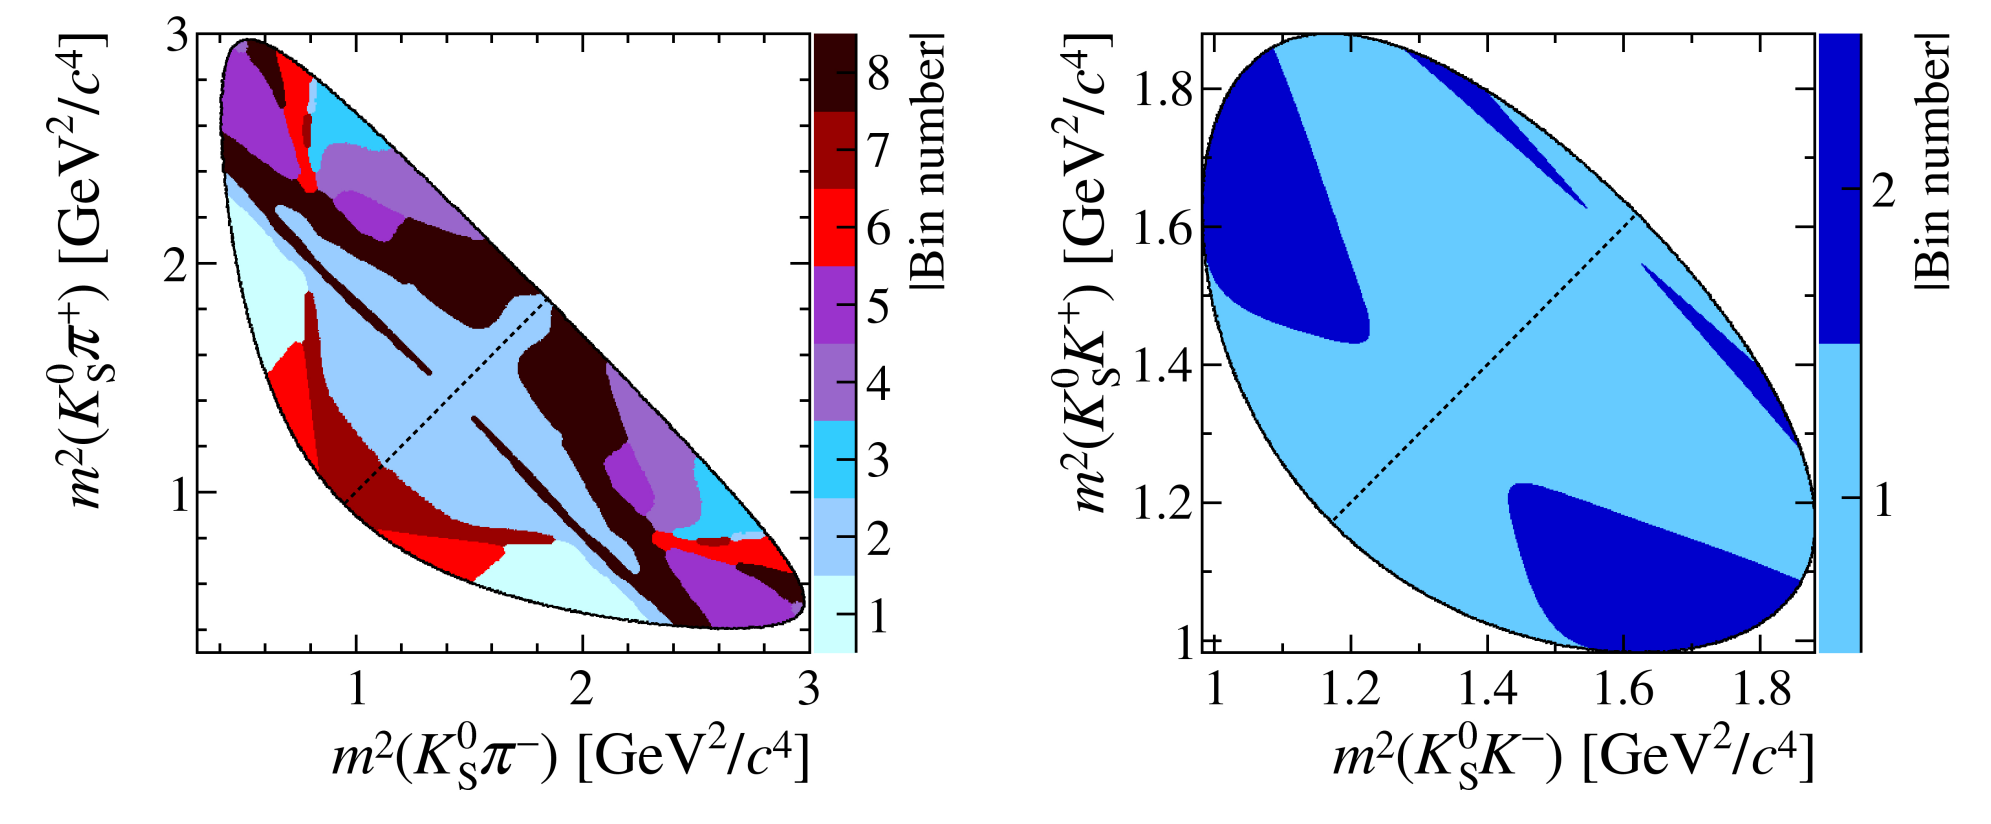
\includegraphics[width=\linewidth]{figures/lect/B2DKstar-Dalitz-binning}
  } \parbox{.45\linewidth}{
    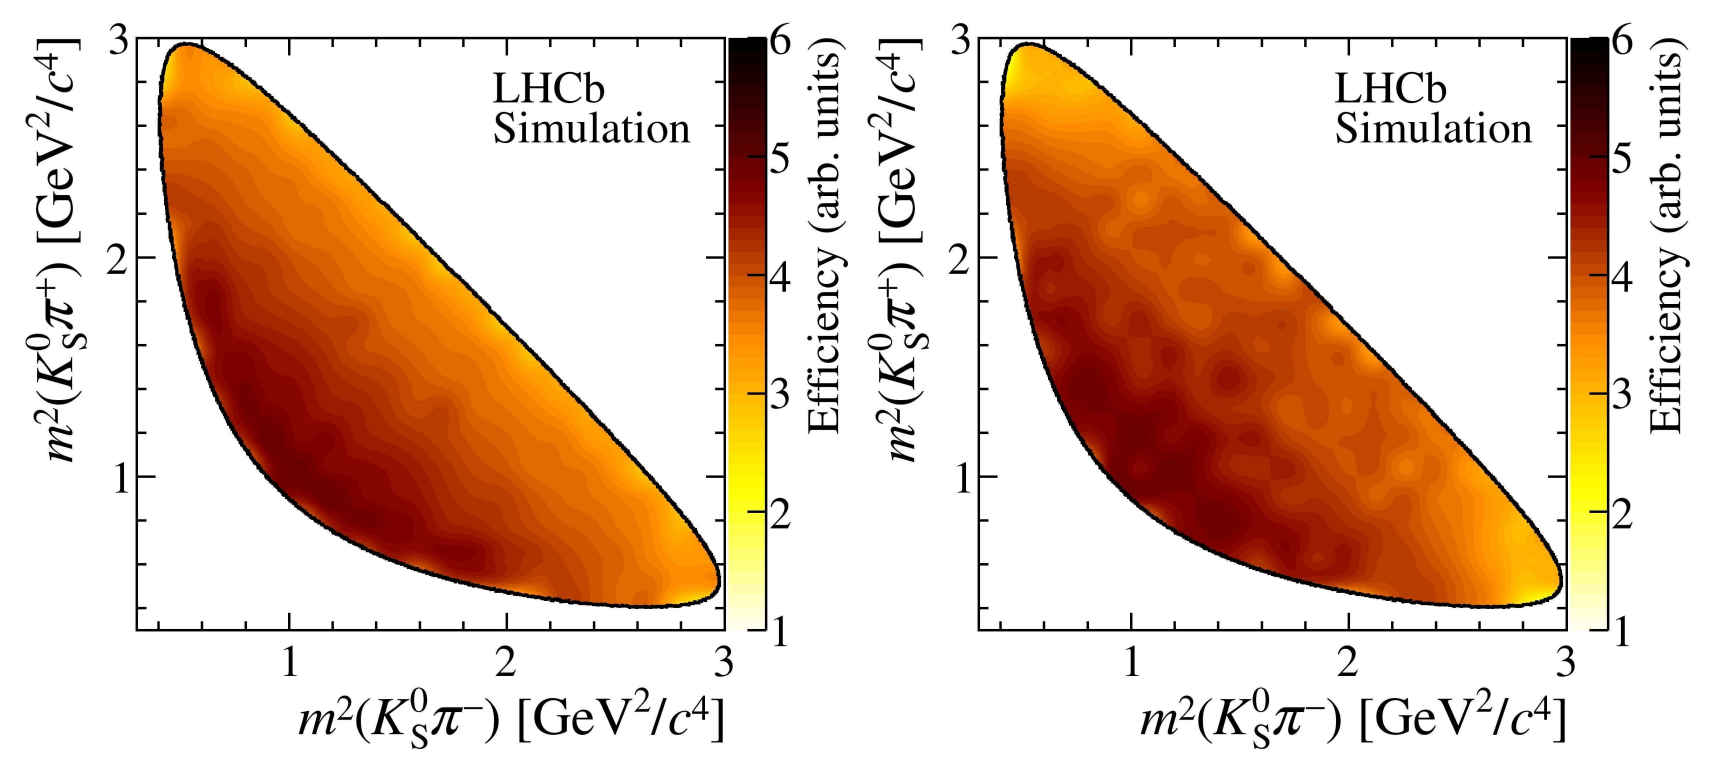
\includegraphics[width=\linewidth]{figures/lect/B2DKstar-eff-Kspipi}
  } \parbox{.45\linewidth}{
    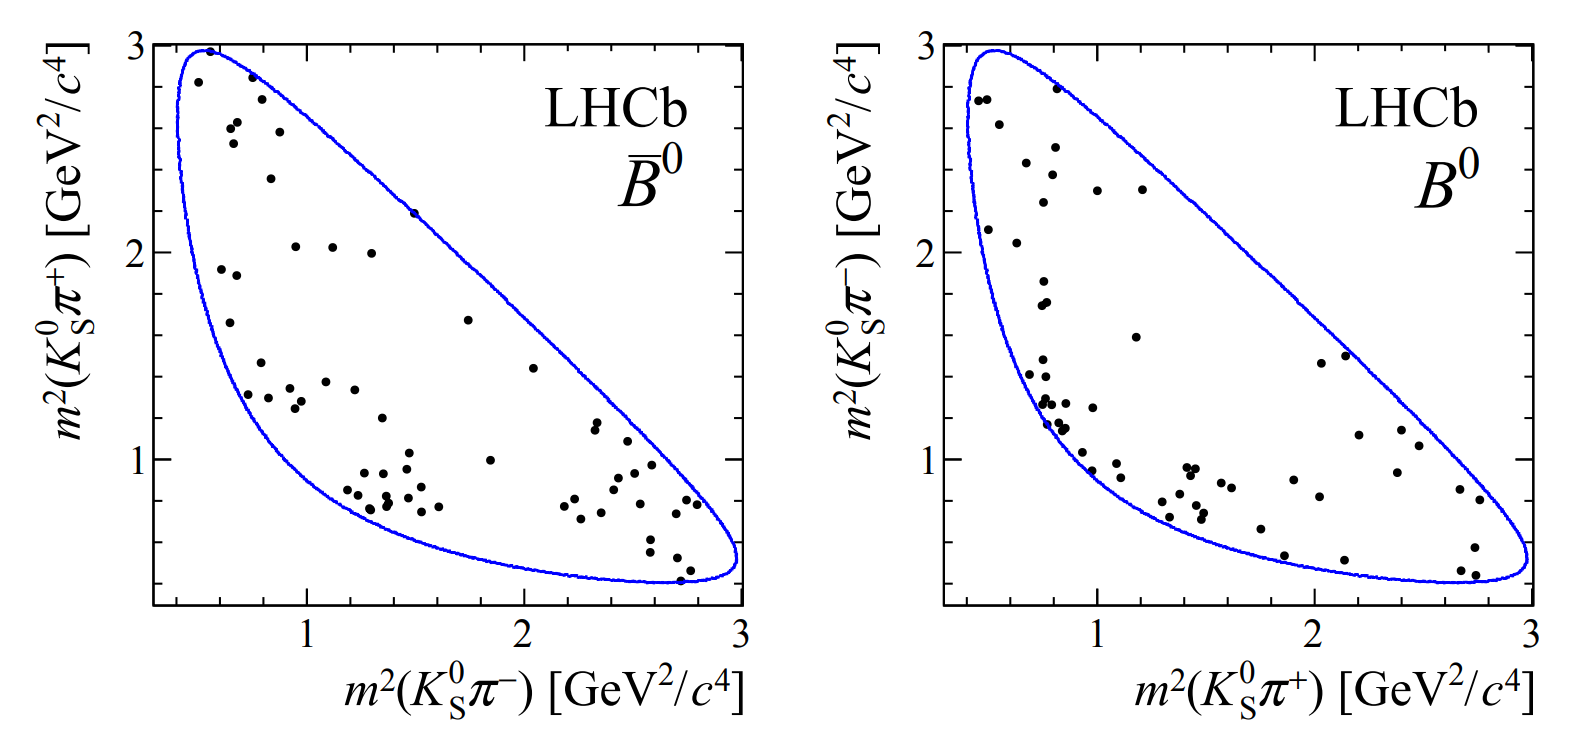
\includegraphics[width=\linewidth]{figures/lect/B2DKstar-Dalitz-Kspipi}
  } \parbox{.45\linewidth}{
    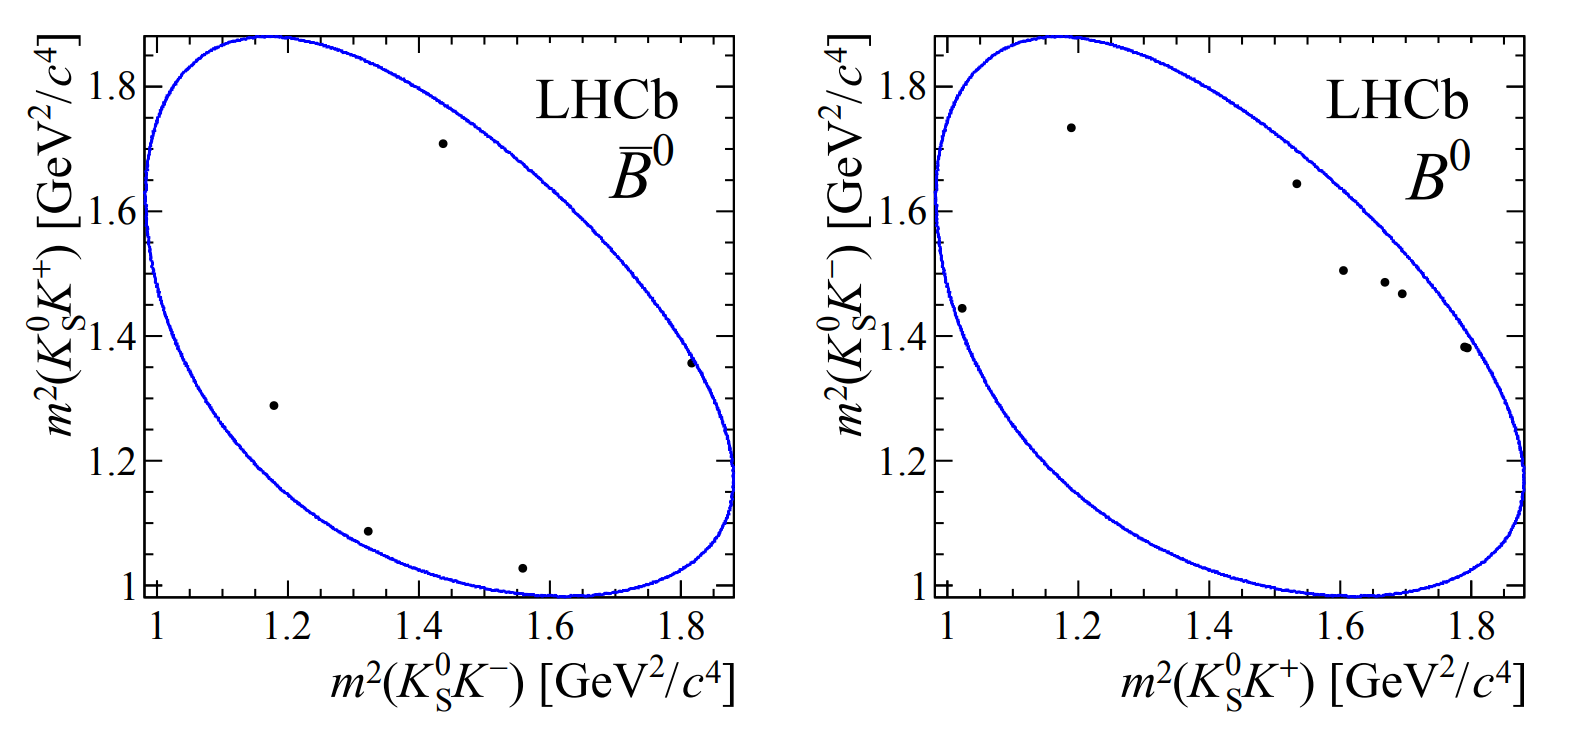
\includegraphics[width=\linewidth]{figures/lect/B2DKstar-Dalitz-KsKK}
  }
\end{frame}%}}}

\begin{frame}[label=B2DKstar-results]%{{{
  \frametitle{$\Bz\to D\Kstarz$ amplitude interference parameters}
  \centering
  \parbox{.34\linewidth}{
    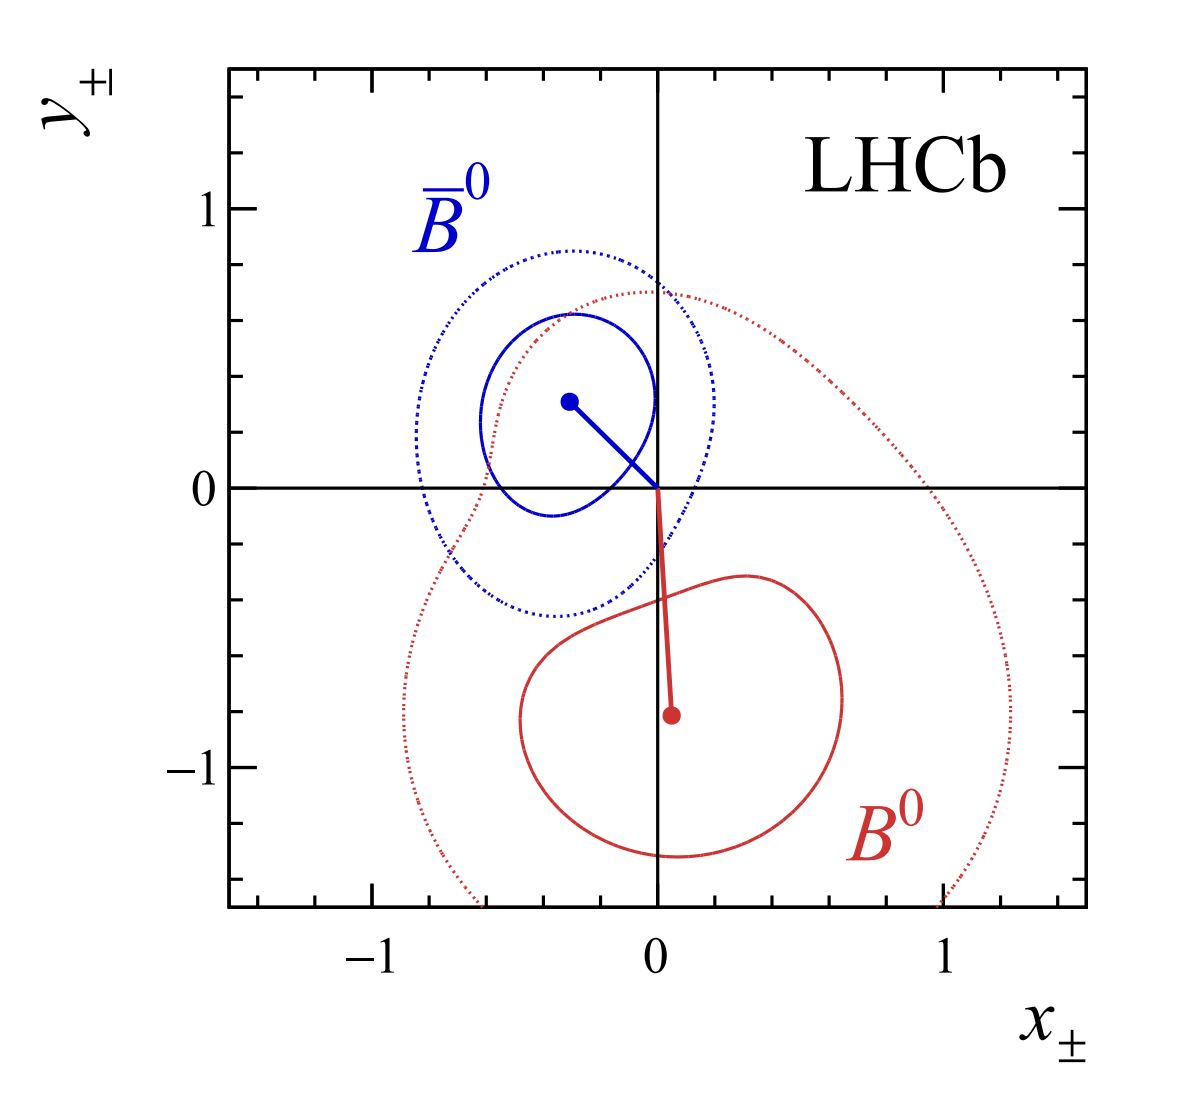
\includegraphics[width=\linewidth]{figures/lect/B2DKstar-results-xy}
  } \parbox{.65\linewidth}{
    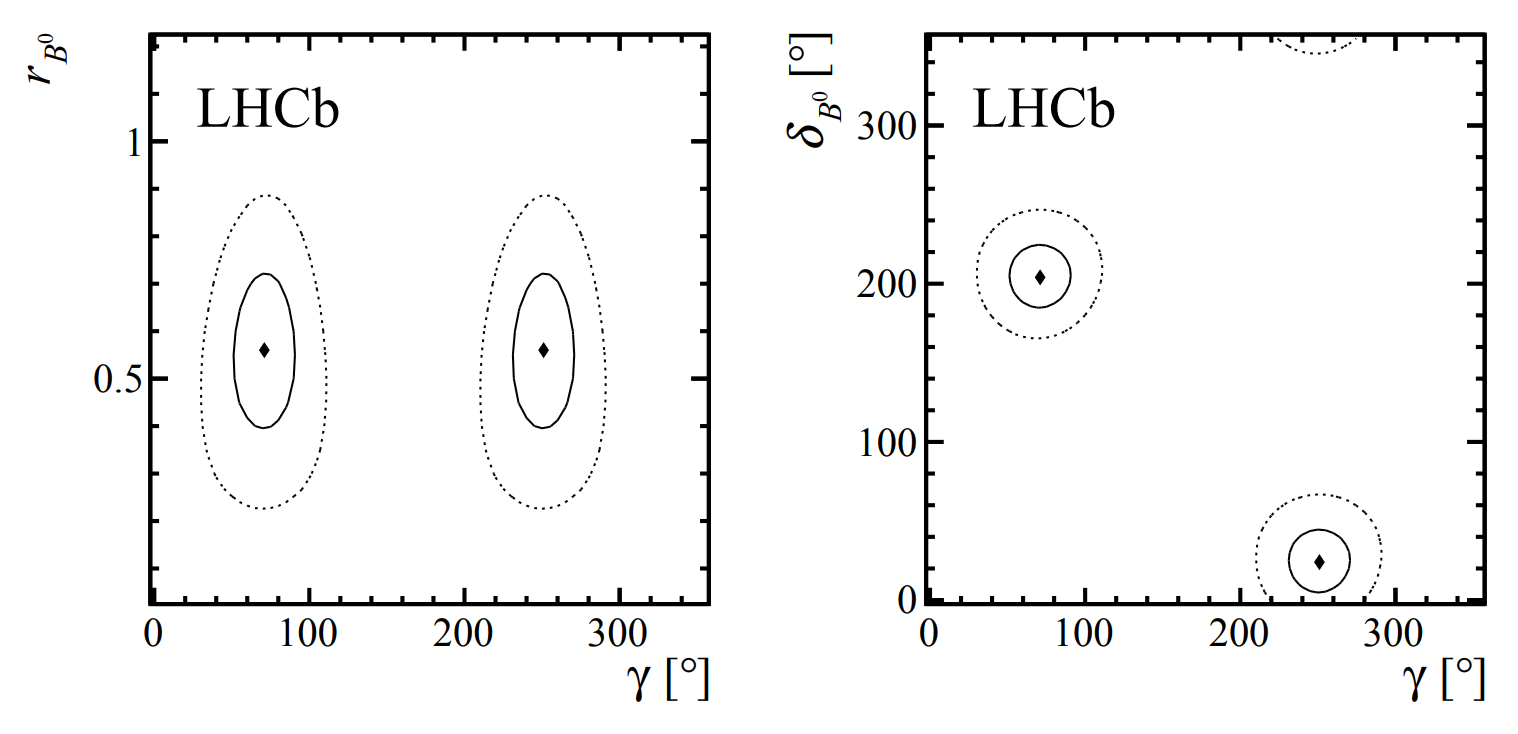
\includegraphics[width=\linewidth]{figures/lect/B2DKstar-results-phys}
  }
  \parbox{.3\linewidth}{
    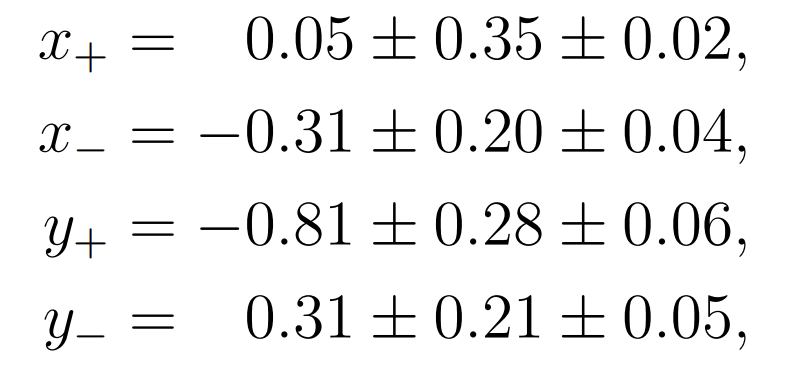
\includegraphics[width=\linewidth]{figures/lect/B2DKstar-results-xy-txt}
  }
  \hspace{4ex}
  \parbox{.2\linewidth}{
    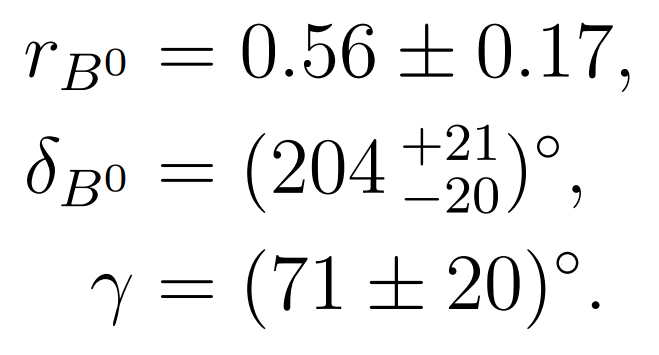
\includegraphics[width=\linewidth]{figures/lect/B2DKstar-results-phys-txt}
  }
  \hspace{4ex}
  \parbox{.2\linewidth}{\centering $\gamma = (65.9\pm3.4)^{\circ}$
  \\ World average}
\end{frame}%}}}

\begin{frame}[label=conclusion]%{{{
  \frametitle{Conclusion}
  \begin{itemize}
    \item First observation of $\Lb \to D\left(\to\Kp\pim\right) p\Km$;
      \\ measurement of its probability relative to
      $\Lb \to D\left(\to\Km\pip\right) p\Km$ (same as expected);
      \\ measurement of its CP asymmetry (consistent with zero).
    \item $\Bz\to D\Kstarz$ with $D\to\Kshort\pip\pim$, $\Kshort\Kp\Km$
      amplitude interference is measured using a~purely data-driven 
      approach.
      \\ The results are independent of other ones and will still 
      contribute to the $\gamma$ measurements despite the worse 
      accuracy.
    \item Upper limit on the probabilities of 16 $B_c^+\to DD$ are 
      improved.
      \\ Evidence of a single one, $B_c^+\to D_s^+\bar{D}^0$, 
      is~reported.
    \item Larger data samples are already on the way.
  \end{itemize}

  \pause \vfill \centering \large Thank you!
\end{frame}%}}}

\end{document}

Mixing of K, D, B, Bs

CP violation with Lb to D meson and other

CP violation only where there's interference

Interference is opposite for antiparticles?

Increased sensitivity in regions with more intermediate resonances

---
The LHCb detector is designed for the study of b- and c-...


---
Bkg from Lb to Lc h with Lc to p h h is excluded by vetoing phh away 
from mLc

Bkg from Lb to p h h h is reduced by requirements on the D decay time.

BDT signal from MC, bkg from exp. Lb sidebands.
Variables: reco kin fit, pid, pT.

Lb region is simply cut out, not weighted.


---
Sim fit of the favored and suppressed decays.

Sums of 2 gaussians, ones with modified tails, bifurcated ones.
Fixed to fit results to the simulation.
Sigmas have a common scale parameter.
The mass difference is fixed for most prominent peaks.
The ratio between components is constrained by BRs and fragmentation.

Dalitz plot and projections show that there are resonances, see text.


---
Fi parameters are determined from semileptonic decays for flavor 
tagging. Their selection is so that the eff. is more like our decay. The 
sample of that decays is somewhat sacrificed, 20\%.
